% !TEX options=--shell-escape
\documentclass[12pt,a4paper]{article}
\usepackage{geometry}
\usepackage[numbers]{natbib}
\usepackage{amssymb, amsmath}
\usepackage{graphicx,wrapfig}
\usepackage{grffile}
\graphicspath{{../Figures/}}
\usepackage{gensymb}
\usepackage[font=small]{caption}
\usepackage[utf8]{inputenc}
\usepackage[english]{babel}
\usepackage{fancyhdr}
\usepackage[raggedright]{titlesec}
\usepackage{subcaption}
\usepackage{multirow}
\usepackage{dirtytalk}
\usepackage{framed}
\usepackage[linesnumbered]{algorithm2e}
\usepackage[pdftex,breaklinks]{hyperref}
\hypersetup{
  colorlinks   = true, 
  urlcolor     = green, %Colour for external hyperlinks
  linkcolor    = blue, %Colour of internal links - changed from blue as using that for new bits
  citecolor   = red %Colour of citations
}

\usepackage{array}
\usepackage{booktabs}
\usepackage{rotating}

\usepackage{color}
\geometry {
  a4paper,
  left = 30mm,
  right = 20mm,
  top = 20mm,
  bottom = 20mm
}
\linespread{1.6}

\usepackage{listings}
% \lstset{frame=tb,
%   language=C++,
%   aboveskip=3mm,
%   belowskip=3mm,
%   showstringspaces=false,
%   columns=flexible,
%   basicstyle={\small\ttfamily},
%   numbers=none,
%   numberstyle=\tiny\color{gray},
%   keywordstyle=\color{blue},
%   commentstyle=\color{dkgreen},
%   stringstyle=\color{red},
%   breaklines=true,
%   breakatwhitespace=true,
%   tabsize=3
% }

\usepackage{minted}

\usepackage{titlesec}
\setcounter{secnumdepth}{4}
\titleformat{\paragraph}
{\normalfont\normalsize\bfseries}{\theparagraph}{1em}{}
\titlespacing*{\paragraph}
{0pt}{3.25ex plus 1ex minus .2ex}{1.5ex plus .2ex}


\newcommand{\comment}[1]{\textcolor{red}{#1}}
\newcommand{\orb}[1]{\textcolor{red}{#1}}
\newcommand{\new}[1]{\textcolor{blue}{#1}}
\newcommand{\code}[1]{\lstinline{#1}}
\newcommand{\terminal}[1]{\mintinline{bash}{#1}}

\pagenumbering{roman}

\begin{document}
\author{Katrina Ashton}

\pagestyle{fancy}
\fancyhf{}
\rhead{\thepage}
\lhead{u5586882}

\begin{titlepage}
\topskip0pt
\vspace*{\fill}
\begin{center}
{\Huge Scene mapping using a RGB-D sensor from an UAV}
\end{center}
\bigskip
\noindent
\textbf{Author:} Katrina Ashton \\
\textbf{Supervisor:} Viorela Ila \\
\textbf{Course:} ENGN4712 Engineering Research and Development Project \\
\textbf{Submission:} \today \\
\vspace*{\fill}
\end{titlepage}

\vspace*{\fill}
\addcontentsline{toc}{section}{	Acknowledgments}
\section*{Acknowledgments}
I'd like to thank my supervisor Viorela Ila for her help and guidance. I would also like to thank Jean-Luc Stevens for helping me set-up my quadcopter and associated code, as well as Alex Martin who created the custom parts for my quadcopter and helped me to assemble it and fix it after crashes.
 
I would also like to thank all of the OpenCV contributors whose registration algorithm implementations I used in this report.
\vspace*{\fill}

\newpage



\addcontentsline{toc}{section}{	Abstract}
\section*{Abstract}
This report investigates data registration techniques for use with data captured from a RealSense D415 RGB-D camera mounted to a quadcopter. Data registration techniques are the backbone of mapping algorithms that use visual odometry, and thus choosing a good registration algorithm is extremely important for these applications. 
 
The RGB-D data for this project is collected from the RealSense camera using the official robot operating system (ROS) package. The estimated trajectory is then evaluated using ground truth data obtained from the Vicon system, which uses a number of infra-red (IR) cameras to track markers attached to the quadcopter. The first part of this project was spent setting up this data collection system -- including building the quadcopter, setting up the software, and calibrating the Vicon system.
 
Three different trajectories are investigated -- a circle, a rectangle and a back-and-forth "lawnmower" trajectory. The circle trajectory provides smooth motion and a high level of overlap between frames, so it is expected that the registration algorithms will perform well for it. The rectangle and lawnmower trajectories are investigated as they decouple the translation and rotation, which allows how well the registration algorithms perform on each type of motion to be investigated. 

% The data is captured from two different scenes. The first has little texture except on two boxes at the center of the scene, this was only used for the circle trajectory as the boxes would not remain in view the whole time for the other trajectories. The second has more texture and is used for all three trajectories.
 
Three different registration methods are then investigated -- the Essential Matrix method, Kabsch and Perspective-n-points (PnP). All of these methods use sparse data where the point correspondences are known, these correspondences are found using a feature detector and matcher on the RGB images. The Essential Matrix method registers two sets of RGB data. Kabsch registers two sets of 3D data. PnP registers one set of 2D data with a set of 3D data.
 
It was found that Kabsch performed very poorly, which is likely at least partially due to the fact that the depth data is quite noisy, and could also be due to poorly chosen RANSAC thresholds. The Essential Matrix method and PnP have similar accuracy, although PnP seemed slightly better at coping with corners. PnP is slower, although that could be partially due to the noisy depth data. Overall if paired with a method for reducing drift the Essential Matrix method seems the best choice when time is a factor. PnP may be better if the depth sensor is less noisy or when time is not critical.

\pagebreak
\tableofcontents

\newpage
\pagenumbering{arabic}
\section{Glossary and Notation}
\label{sec: g and n}
\subsection{Abbreviations}
\label{ssec: abb}
ICP: iterative closest point -- a data registration method. \\
IR: infra-red \\
PnP: perspective-n-point \\
RANSAC: random sample consensus (algorithm) \\
RGB-D: red, green, blue, depth --- an RGB-D sensor gives a colour image (red green and blue channels) as well as the associated depth image. \\
ROS: robot operating system. \\
SLAM: simultaneous localization and mapping \\
UAV: unmanned aerial vehicle. 

\subsection{Glossary}
\label{ssec: gloss}
Pose: position and orientation.

\subsection{Notation}
\label{ssec: not}
${}_iT_j$: transformation between frame $i$ and frame $j$, defined in the coordinate system for frame $i$. \\
${}^fT_j$: pose of frame $j$, defined in the coordinate system for frame $f$.


\pagebreak
\section{Introduction}
  \label{sec: intro}
  Being able to create a map of a scene using a robot is useful for a variety of applications -- for example, in aiding the robot in navigating, or in task execution. Using an RGB-D sensor allows depth information to be obtained directly, rather than using techniques such as optical flow or structure from motion. However, even when using an RGB-D sensor, creating an accurate scene map is not always a trivial task due to difficulties in aligning the data and noise in the depth measurements.
   
  A key step in creating scene map from RGB-D data is data registration. Data registration is the process of combining two frames of data, when the relative pose of the camera is not known (or not with certainty). In order for this to work properly there needs to be sufficient degree of overlap between the frames for the algorithm the align them. Ideally data registration should discard noisy or redundant points. There are a number of data registration techniques that work well with noise-less data and will be used as a starting point for this report. These include finding the Essential Matrix (Section \ref{ssec: BI EM}) and using the Kabsch algorithm (Section \ref{ssec: BI kabsch}) and using a method for solving the Perspective-n-points (PnP problem) (Section \ref{ssec: BI PnP}).
   
  This report will focus on data registration for data captured using unmanned aerial vehicles (UAVs). UAVs are very maneuverable and the fact that they travel through the air means that their mobility is independent of terrain. Thus UAVs are highly suitable for mapping tasks, especially when the environment being mapped has rough or uneven ground (e.g. most outside locations) or many obstacles on the ground (e.g. many indoors locations which often have things such as desks and chairs).
   
  A quadcopter was thus built for the purpose of obtaining the necessary experimental data (see Section \ref{sec: quad set-up}), with an attached RealSense camera used to take the RGB-D measurements. The RealSense camera was chosen due to its small size (allowing it to fit on the quadcopter without impacting mobility or flight-time too much) and relatively good quality images. This UAV was then flown under a few different trajectories for different scenes (see Section \ref{sec: data collection}), with ground truth data on the UAV's pose will be obtained using a Vicon localization system (see Section \ref{ssec: BI vicon}). 
   
  Data from a sensor mounted to a UAV is often very noisy due to the fact that the sensor experiences a large amount of shake and rapid motions. The rapid motions can also make it difficult to accurately estimate the difference in pose between measurements. These factors make it difficult to accurately register data. Thus this report aims to design and implement a data registration technique that can perform well in this situation, so that the registered data can be used to form an accurate scene map.

\section{Literature Review}
  \label{sec: LR}

  \subsection{Mapping -- SLAM}
    \label{ssec: LR SLAM}
    Simultaneous Localization and Mapping (SLAM) is a problem for which the aim is for a mobile robot to create a map of its environment while simultaneously determining its location within this map (without prior knowledge of its environment or location). 
     
    There are three main parts to SLAM. The first is obtaining measurements of how the robot is moving (rotation and translation), as well as data it sense from the environment. These measurements then need to be used to update both the robot's map of the environment and its estimate of its position in it. Finally, almost all SLAM implementations have some way of detecting when the robot senses a feature or returns to a place more than once, and using this to update the estimate of the map and the robot's location. This last step is important for reducing the effect of drift that generally occurs when mapping.
     
    The first step, obtaining the measurements of how the robot is moving, may seem relatively simple, and indeed some robots are equipped with sensors such as rotary encoders and gyroscopes that give relatively accurate and precise measurements of the robot's movements with minimal calibration. However, not all robots can be equipped with such sensors (e.g. quadcopters do not have wheels and thus cannot use rotary encoders) and so have to rely on sensors such as cameras, which require much more computation to get useful measurements. How to estimate the motion of a camera from sequential frames (known as data registration) is an ongoing area of research.
     
    Henry et al \citep{henry2012rgb} use a Kinect RGB-D camera to perform dense 3D modeling of indoor environments using SLAM. For their data registration, they use a variant of the iterative closet point (ICP) algorithm, which they call RGB-D ICP, as part of their RGB-D mapping system. This algorithm first finds an estimated transform, and then refines it using ICP. This initial estimate is found using sparse point clouds, created by extracting features from the RGB images, matching them between frames, and then using them along with their corresponding depth measurements to form 3D points. It proposes two ways to find the transform from these sparse point clouds, depending on the type of sensor used to capture the RGB-D data. For time-of-flight cameras, it optimizes for point-to-point squared distance error, using the method of Horn \citep{horn1988closed}, which uses quaternions to find the optimal rotation. For active stereo RGB-D cameras it optimizes for re-projection error, using two-frame sparse bundle adjustment (SBA). In both cases, Random Sample Consensus (RANSAC) is used in conjunction with these methods to try to remove outliers. This estimated transform is then used as the initial estimate for ICP, again in conjunction with RANSAC, but this time on dense point clouds rather than the sparse ones. The version of RANSAC used is point-to-plane, with minimization using Levenberg-Marquardt. They found that doing the ICP step only gave marginal improvements if sufficient RANSAC inliers were found during the initial estimate. Thus they only performed ICP when the number of inliers found was below a certain threshold.
     
    Kerl et al \citep{kerl2013dense} perform dense visual SLAM on RGB-D data from the {RGB-D SLAM} Dataset and Benchmark \cite{dataset}, which is also captured using a Kinect, and contains a few different indoor environments. They use joint photometric and geometric error minimization for their data registration. It does this by modeling the photometric error and depth error as a bivariate random variable which follows a bivariate t-distribution. This defines an error function which can then be linearized using a first order Taylor expansion, and then solved iteratively.
     
    Mur-Artal et al's ORB-SLAM \cite{mur2015orb} performs feature-based monocular SLAM on three different datasets, one from a robot, one hand-held and one from a car. (The NewCollege dataset \cite{smith2009new}, TUM RGB-D benchmark \cite{sturm2012benchmark} and KITTI dataset \cite{geiger2013vision}, respectively). This method uses ORB features \cite{rublee2011orb} as they are fast and rotation invariant. For data registration, they compute two geometrical models: a homography assuming a planar scene and a fundamental matrix assuming a non-planar scene. It chooses between these scenes by calculating a score for each and using a heuristic a ration between them. ORB-SLAM tracks the camera's pose in the local map. When tracking is lost it uses the PnP algorithm to relocalize the camera. 


  \subsection{RGB-D data registration -- ICP}
    \label{ssec: LR ICP}
    One of the most common methods for data registration is the iterative closest point (ICP) method, of which there are many variations \cite{pomerleau2013comparing}. ICP is only used on two 3D models at a time, and an initial estimate of the relative pose between these two models must be known \cite{rusinkiewicz2001efficient}. ICP can be used on either dense or sparse point clouds.
     
    \citet{rusinkiewicz2001efficient} identify six stages of the ICP algorithm:
    \begin{enumerate}
    \item{\textbf{Selection} of some set of points in one or both models}
    \item{\textbf{Matching} the selected points between the two models}
    \item{\textbf{Weighing} the corresponding point pairs}
    \item{\textbf{Rejecting} certain pairs (can be done by either looking at pairs individually or considering the entire set of pairs)}
    \item{Assigning an \textbf{error metric} based on the pair points}
    \item{\textbf{Minimizing} the error metric}
    \end{enumerate}
    The variants of ICP affect one or more of these stages.
     
    The matching step is generally done in the Euclidean space using kd-tree to accelerate the search \cite{pomerleau2013comparing}. The most common distance measures used for the matching step are point-to-point and point-to-plane \cite{pomerleau2013comparing}. Point-to-plane was created to deal with the fact that taking a measurement of a surface imposes a discretization error, it does this by not penalizing offsets along a surface \cite{segal2009generalized}.
     
    % The algorithm itself is not the only thing that impacts the performance of ICP. The sensor used to capture the data can have a large impact, depending on its noise, field of view and point density inside the field of view \cite{pomerleau2013comparing}. Having less noise means less outliers and thus better results. Having a wide field of view with a high density of points leads to more overlap and a higher probability of multiple matching points. ICP also performs better in unstructured environments and with more accurate information on starting positions and movement. 
    %  
    Generalized ICP (GICP) \cite{segal2009generalized} combines the point-to-point and point-to-plane methods to model a locally planar surface in both scans, a technique they say can be thought of as plane-to-plane. GICP focuses on the error metric and minimization steps. It uses a probabilistic model where the points in each point cloud are assumed to be drawn from independent Gaussians, then Maximum Likelihood Estimation (MLE) is used to find the transformation.
     
    When used in SLAM, ICP generally seems to be used to refine pose estimations rather than as the sole registration technique \cite{engelhard2011real,henry2012rgb}.


  \subsection{RGB data registration -- Photometric error}
    \label{ssec: LR photmetric}
    One popular method for dense RGB image registration is minimizing photometric error \cite{kerl2013dense,bartoli2008groupwise,newcombe2011dtam}. Photometric error is a measure of photo-consistency, i.e. how well the points in an image and another aligned image agree. 
     
    When depth data is available, the geometric error is often used in conjunction with the photometric error. There are also a few variants of geometric error that can be used, the main ones being Euclidean (as in ICP) and re-projection (which is similar to photometric error but for the depth map rather than the RGB image). There are also a few different approaches to combining the photometric error and geometric error into a unified error function. For example, include using a weighted sum of a non-linear function of each error (e.g. sigmoid) \cite{morency2002stereo}, and forming a bivariate random variable and using that to define an error function \cite{kerl2013dense}.

  \subsection{RGB data registration -- Essential Matrix}
    \label{ssec: LR EM}
    The Essential Matrix method works on RGB data from a calibrated camera with known point correspondences. It first uses the point correspondences and the camera calibration parameters to find the Essential Matrix, and then uses the Essential Matrix in conjunction with the point correspondences to find the change in camera pose. The original method was proposed by Longuet-Higgins \cite{longuet1981computer} and gives a closed-form solution for 8 point correspondences. Iterative methods for solving this problem were also developed \cite{haralick1989pose}, but it was found that a slight modification to the closed form solution made its results competitive with iterative algorithms while being much faster \cite{hartley1995defence}. More recently, an efficient 5-point closed form algorithm has been developed that is now widely used \cite{nister2003efficient}.
     
    ORB-SLAM \cite{mur2015orb} uses the Essential Matrix, which they find from the Fundamental Matrix, for registration when the scene is non-planar and has high parallax. When the scene is planar, nearly planar or there is low parallax, a Fundamental Matrix can be found but the problem is not well constrained, and thus ORB-SLAM uses homography instead for these cases.

  \subsection{RGB-D data registration -- Kabsch}
    \label{ssec: Kabsch}
    The Kabsch algorithm was first proposed in 1976 by Kabsch \cite{kabsch1976solution} as a way of aligning two sets of matched 3D points, with an amendment two years later which ensures a proper rotation is obtained \cite{kabsch1978discussion}. The original formulation is in terms of Lagrange multipliers, but modern implementations use singular value decomposition (SVD) \cite{kavraki2009geometric}.
     
    The Kabsch algorithm is fairly widely used for aligning molecules \cite{kavraki2009geometric,goldschmidt2010identifying} and indexing rotation diffraction patterns \cite{kabsch1988automatic,kabsch2010xds}. More recently, it has been used by the computer vision community on RGB-D data as part of tasks such as non-rigid reconstruction \cite{zollhofer2014real}, pose estimation \cite{brachmann2014learning} and camera re-localization \cite{shotton2013scene}. 

  \subsection{RGB-D data registration -- Perspective-n-Point}
    \label{ssec: PnP}
    The Perspective-n-Point (PnP) problem is to determine the pose of a calibrated camera given a set of $n$ correspondences between 3D points and their 2D projections. The term PnP problem was introduced by Fischler and Bolles \cite{fischler1981random}, as reformulation of the Location Determination Problem. The PnP problem is only solvable for $n \geq 3$, however for $n=3$ there are multiple viable solutions, so a fourth point correspondence is needed to remove ambiguity. A widely accepted solution to the P3P problem is given in Gao et al \cite{gao2003complete}. For arbitrary $n\geq 4$, there are various iterative methods \cite{oberkampf1996iterative,haralick1989pose}, as well as an $O(n)$ closed-form solution called EPnP \cite{lepetit2009epnp}.    
     
    EPnP is used in ORB-SLAM \cite{mur2015orb} to relocalize the camera when tracking is lost.


\section{Background}
  \label{sec: BI}
  This section details the necessary background information on rigid body motion, coordinate frames, the pinhole camera model and registration methods. The registration methods described in Sections \ref{ssec: BI EM}-\ref{ssec: BI PnP} are key to this report, as it focuses on comparing them for use with data from a quadcopter. These methods are all used in conjunction with the Random Sample Consensus (RANSAC) algorithm in order to reduce the effect of outliers, and so the RANSAC algorithm is described in Section \ref{ssec: BI RANSAC}.
   
  However, before these algorithms can be properly implemented and used for mapping, an understanding of how the quadcopter can move, as well as coordinate frames and how to convert between the image and camera frames is necessary. Thus, Section \ref{ssec: BI motion} describes the basics of rigid body motion, Section \ref{ssec: BI coord} describes the relevant coordinate frames and how to convert between them, and Section \ref{ssec: BI camera model} describes the camera model used, its intrinsic parameters and also derives the equations used to convert between the image and camera frames.
   
  The Essential Matrix (Section \ref{ssec: BI EM}), Kabsch (Section \ref{ssec: BI kabsch}) and Perspective-n-Points (PnP) (Section \ref{ssec: BI PnP}) methods all represent fairly basic algorithms that can be used on sparse data where the point correspondences are known. The simplest way to get such data is to use a feature detector and then match the features between the frames being registered. Each of these methods uses data from different frames: the Essential Matrix uses data from image frames (RGB), Kabsch uses data from camera frames (3D) and PnP takes data from an image frame (RGB) and data from a camera frame (3D).
   
  Many of these algorithms are already implemented in the Open Source Computer Vision Library (OpenCV) and where available these implementations are used in this report. Thus an overview of OpenCV and how to use it is provided in Section \ref{ssec: BI OpenCV}.

  \subsection{Rigid Body Motion}
    \label{ssec: BI motion}
    Rigid body motion is motion of a body that preserves the Euclidean distance between any two points on that body. There are three types of rigid body motion: rotations, translations and reflections, with a combination of the three also being a rigid body motion. Proper rigid body motion also specifies that handedness is preserved, which excluded reflections. This report only considers proper 3D rigid body motion, i.e. combinations of rotation and translation in 3 dimensions.
     
    When applied to a body, a rotation and translation change its orientation and position, respectively. Together orientation and position are called \textit{pose}. Proper rigid body motion and poses are both elements of the Special Euclidean Group $SE(3)$, although they are generally represented as members of its associated Lie Algebra $\mathfrak{se}(3)$ which decouples the rotation and translation.
     
    There are multiple ways of representing a rotation. One way is a rotation matrix, which is an element of the Special Orthogonal group $SO(3)$, that is it is an orthogonal $3\times 3$ matrix with determinant 1. Another way is by axis-angle, which gives an axis about which the rotation occurs (unit vector in $\mathbb{R}^3$) and the magnitude of that rotation (element of $\mathbb{R}$). Another common way is with Quaternions, which can be written as $(a,b,c,d) \in \mathbb{R}^4$ which represents the Quaternion $a+b\textbf{i} + c\textbf{j} + d\textbf{k}$ where $\textbf{i}, \textbf{j}, \textbf{k}$ are the fundamental Quaternion units with the property that $\textbf{i}^2=\textbf{j}^2=\textbf{k}^2=\textbf{ijk}=-1$. Rotation matrices and Quaternions are easier to combine and apply to a body than axis-angle, with Quaternions being more compact and generally being faster to compute than rotation matrices. The axis angle representation is useful for comparing rotations, e.g. for finding errors, they are not over parameterized. 
     
    Translations are elements of $\mathbb{R}^3$; range and bearing can also be used to represent them.



  \subsection{Coordinate frames}
    \label{ssec: BI coord}
    There are four main coordinate frames relevant to this report: the world-fixed frame, the quadcopter-fixed frame, the camera-fixed frame and the image-fixed frame. The "fixed" part of these names may be dropped (so camera frame refers to the camera-fixed frame). There is also another world-fixed frame that the ground truth position data is given in, this will always be referred to as the quadcopter world-fixed frame (which is not the same thing as the quadcopter-fixed frame). This report seeks to use RGB-D information in the image frame to find the movement of the camera in the world frame, but to do this the camera frame and then quadcopter frame must be passed through. An additional Vicon frame is defined, which is the format that the ground truth poses of the quadcopter are given in (see Section \ref{sec: data collection}). The Vicon frame could be used as the world reference frame, however for ease of plotting and understanding it was decided to use two frames. Figure \ref{f: frames} shows these frames and how they relate to each other. 

    \begin{figure}[b!]
      \centering
        \includegraphics[width=120mm, trim = 30mm 40mm 70mm 50mm, clip]{frames/frames_env.pdf}
      \caption{(Best viewed in colour). 3D coordinate frames and how they relate. World frame $\{W\}$ in green, Vicon frame $\{V\}$ in purple, quadcopter frame $\{Q\}$ in blue, camera frame $\{C\}$ in orange.}
      \label{f: frames}
    \end{figure}

    Before continuing further, notation for poses and transformations is necessary. Let ${}^fT_j$ be the pose of frame $j$, defined in the coordinate system from frame $f$. Then let ${}_iT_j$ be a transformation between frame $i$ and frame $j$, defined in the coordinate system for frame $i$. These frames can be represented by just a letter $W$ for world, $Q$ for quadcopter, $C$ for camera, $I$ for image, and $V$ for Vicon. However, the camera and quadcopter frames are not fixed with respect to the world frame, so the timestep needs to be given as well. So $Qn$ refers to the quadcopter frame at the $n^{\text{th}}$ timestep, and likewise $Cn$ refers to the camera frame at the $n^{\text{th}}$ timestep.
     
    The ground truth position data is in the Vicon frame (with the $x$-axis aligned with the world frame), and so needs to be converted to the world frame. This can be done by multiplying it by a rotation matrix, ${}_VR_W$ which rotates by 180 degrees around the $x$-axis.
     
    The registration finds transforms in the camera frame, which then need to be converted into the world frame. To convert from the camera to world frame, the quadcopter-fixed frame is passed through and the pose of the quadcopter-fixed frame in the world frame must be known. To convert from the camera frame to the quadcopter frame another rotation matrix, ${}_CR_Q$ is used, this rotation matrix first rotates around the $x$-axis by 135 degrees, then about the (new) $z$-axis by 90 degrees. Looking at Figure \ref{f: frames}, it can be seen that these rotations will take the camera frame (orange) into alignment with the the quadcopter frame (blue). Note that the camera is not actually mounted to the center of the quadcopter, so an accurate transformation would include some translation along with the rotation. However, the center of the quadcopter in the ground truth is defined by the Vicon, and is difficult to locate it and measure the distance to the camera precisely. The Vicon also often needs to be re-calibrated, which may result in the point defined as the center changing slightly. In addition, the magnitude of the translation is also not very large, thus it was decided that the benefit of including a translation in the transform did not outweigh the added complications.
     
    Then, when ${}^W[R|t]_{Qn}$ and ${}_{Cn}[R|t]_{C(n+1)}$ are known, ${}^W[R|t]_{Q(n+1)}$ is obtained as follows:
    \begin{align*}
    ^{W}R_{Q(n+1)} &= {}^{C0}R_{Qn} \: {}_CR_Q \: {}_{Cn}R_{C(n+1)} \: {}_CR_Q^T \\
    ^Wt_{Q(n+1)} &= {}^WR_{Qn} + {}^WR_{Qn}^T \: {}_CR_Q \: {}_{Cn} t_{C(n+1)} 
    \end{align*}

    \bigskip \noindent
    In order to use these equations, the first pose ${}^W[R|t]_{Q0}$ is assumed to be known (in this report it is taken from the ground truth, some other methods initialize at the origin). Then there are two possible methods to find ${}^W[R|t]_{Q(n+1)}$. The first is by finding an absolute estimated transform. In this case, the previous estimate is used for ${}^W[R|t]_{Qn}$ (so the estimations must be done from the first timestep to the $n+1^{\text{th}}$ timestep in order to get the absolute estimated transform ${}^W[R|t]_{Q(n+1)}$). The second is to get a relative estimated transform. In this case, the ground truth is used for ${}^W[R|t]_{Qn}$ (so only ${}_{Cn}[R|t]_{C(n+1)}$ needs to be found to get the absolute estimated transform ${}^W[R|t]_{Q(n+1)}$). The absolute trajectory is what will be used in practice in most cases (as the ground truth is not known). However the absolute error is prone to drift, so looking at the relative error can give a better insight into how accurate the registration is at each timestep (and thus give insight into possible sources of error).

    %code
      % R_rgb = np.dot(Rc2q,np.dot(R_rgb,Rc2q.transpose()))
      % t_rgb = np.dot(Rc2q,t_rgb)

      % q_c = np.dot(rot_rgb, R_rgb)
      % pos_rgb = pos_rgb + np.transpose(np.dot(Rq2w, np.dot(rot_rgb.transpose(),t_rgb))) #first one is in global frame, so don't rotate
      % rot_rgb = q_c

      % qr = np.dot(Rq, R_rgb)
      % rpos_rgb = pq + np.transpose(np.dot(Rq2w, np.dot(Rq.transpose(),t_rgb))) 

  \subsection{Camera model}
    \label{ssec: BI camera model}
    This report uses a pinhole camera model, which is equivalent to assuming no lens or aperture distortion. It is also valid when distortion is removed from image data during preprocessing. 
    \begin{figure}[h]
    \centering
      \includegraphics[height=100mm, trim = 50mm 10mm 50mm 10mm, clip]{diags/pinhole.pdf}
    \caption{(Best viewed in colour). Pinhole camera model}
    \label{fig: pinhole}
    \end{figure}
    Under the pinhole model, the scene view is formed by projecting 3D points into the image plane using the perspective transformation \cite{OpenCV-3d-reconstruction}
    \[
    sm' = K[R|t] M'
    \]
    which is
    \[
    s \begin{bmatrix} u \\ v \\ 1 \end{bmatrix} = \begin{bmatrix} f_x & 0 & c_x \\ 0 & f_y & c_y \\ 0 & 0 & 1 \end{bmatrix} \begin{bmatrix} r_{11} & r_{12} & r_{13} & t_1 \\ r_{21} & r_{22} & r_{23} & t_2 \\ r_{31} & r_{32} & r_{33} & t_3 \end{bmatrix} \begin{bmatrix} X \\ Y \\ Z \\ 1 \end{bmatrix}
    \]
    where 
    \begin{itemize}
      \item $(X,Y,Z)$ are the coordinates of a 3D point in the world frame
      \item $(u,v)$ are the coordinates of the corresponding projection point in pixels (image coordinates)
      \item $s$ is a scaling term
      \item $R$ and $t$ are a rotation and translation matrix of the camera, respectively
      \item $K$ is a matrix of intrinsic camera parameters (note that there is no skew term due to the fact that a pinhole camera model is used)
      \item $(c_x, c_y)$ is the principal point (usually at the image center), see Figure \ref{fig: pinhole}
      \item $f_x$ and $f_y$ are the focal lengths expressed in pixel units. Figure \ref{fig: pinhole} shows the case where $f=f_x=f_y$ as in an ideal pinhole camera, but this is not necessarily the case in practice. When $f_x \neq f_y$, the resulting image has non-square pixels.
    \end{itemize}
    This can be written in a way that is easier to switch between the image and camera frames. Start by inverting $K$:
    \[
    K^{-1} = \begin{bmatrix} 1/f_x & 0 & -c_x/f_x \\ 0 & 1/f_y & -c_y/f_y \\ 0 & 0 & 1 \end{bmatrix}
    \]
    And $[R|t] [X Y Z 1]^T = R [X Y Z]^T + t$, so
    \begin{align*}
    s \begin{bmatrix} u \\ v \\ 1 \end{bmatrix} &= \begin{bmatrix} f_x & 0 & c_x \\ 0 & f_y & c_y \\ 0 & 0 & 1 \end{bmatrix} \begin{bmatrix} r_{11} & r_{12} & r_{13} & t_1 \\ r_{21} & r_{22} & r_{23} & t_2 \\ r_{31} & r_{32} & r_{33} & t_3 \end{bmatrix} \begin{bmatrix} X \\ Y \\ Z \end{bmatrix} \\
    s \begin{bmatrix} 1/f_x & 0 & -c_x/f_x \\ 0 & 1/f_y & -c_y/f_y \\ 0 & 0 & 1 \end{bmatrix}\begin{bmatrix} u \\ v \\ 1 \end{bmatrix} &= R \begin{bmatrix} X \\ Y \\ Z \end{bmatrix} + t \\
    s \begin{bmatrix} u/f_x - c_x/f_x \\ v/f_y - c_y/f_y \\ 1 \end{bmatrix} &= R \begin{bmatrix} X \\ Y \\ Z \end{bmatrix} + t \\
    \begin{bmatrix} s(u-c_x)/f_x \\ s(v-c_y)/f_y \\ s \end{bmatrix} &= R \begin{bmatrix} X \\ Y \\ Z \end{bmatrix} + t 
    \end{align*}
    Note that $R \begin{bmatrix} X \\ Y \\ Z \end{bmatrix} + t $ is the position of a 3D point in the camera frame. So this gives
    \begin{align*}
    x &= s(u-c_x)/f_x \\
    y &= s(v-c_y)/f_y \\
    z &= s
    \end{align*}
    and thus
    \begin{align*}
    u &= xf_x/z + c_x \\
    v &= yf_y/z + c_y
    \end{align*}    
    for a point $(x,y,z)$ in camera coordinates with projected image coordinates $(u,v)$. 
     
    This can be written as the projection function 
    \begin{align*}
    \pi(^I\textbf{p}) = (s(u-c_x)/f_x, s(v-c_y)/f_y, s)
    \end{align*}
    and inverse projection function
    \begin{align*}
    \pi^{-1}(^C\textbf{p}) = (xf_x/z + c_x, yf_y/z + c_y)
    \end{align*}
    for a point $^c\textbf{p} = (x,y,z)$ in the camera frame with projected image coordinates $^i\textbf{p} = (u,v)$. These functions require that the principal point, focal lengths and scaling factor of the camera are known. This report only works with calibrated cameras, so these functions can be used.

  \subsection{OpenCV}
    \label{ssec: BI OpenCV}
    The Open Source Computer Vision Library (OpenCV) is a library with C++, Python and Java interfaces which provides a number of useful functions for working with images and performing computer vision tasks \cite{openCV}. It implements the Essential Matrix method and PnP, as well as a feature descriptor and matcher. OpenCV is well established, widely used and has many contributors, thus these functions are likely well optimized. OpenCV is also implemented in C/C++ code, with an interface provided for use with other languages, thus their implementation will also likely be faster than a purely Python implementation would be. Therefore when OpenCV implementations of functions are available they will be used instead of coding them from scratch.
     
    In Windows, OpenCV for Python can be installed via pip (\terminal{pip install opencv-python}). There are also anaconda distributions as well as official releases with pre-built binaries and source code. After OpenCV is installed, it can be imported using \terminal{import cv2}. 
     
    The main OpenCV functions used in this report are described in the Camera Calibration and 3D Reconstruction documentation \cite{openCV-docs}. OpenCV also provides various feature descriptors (such as SIFT, SURF, ORB, BRIEF, BRISK) and functions for matching features (such as FLANN and a brute force matcher) \cite{openCV-feat}. This report uses the SIFT feature descriptor, and the matches are found using a brute force matcher.

  \subsection{RANSAC}
    \label{ssec: BI RANSAC}
    The RANdom SAmple Consensus (RANSAC) algorithm is method of fitting a model to data with a high proportion of outliers. Previous techniques for dealing with outliers often started by using all of the data and then trying to remove wrong correspondences, RANSAC takes the opposite approach of starting with a small number of points and adding data that is consistent with the model generated from these points \cite{fischler1981random}. It begins by sampling the minimum number of points needed to find parameters for the model, and finds parameters based only on those points. It then finds all the points that are consistent with the model using those parameters (up to some predefined tolerance). If there are enough points (i.e. the proportion is over some other predefined threshold), the parameters are re-estimated using all of the consistent points. If there are not enough points, the process begins again by sampling new points. A maximum number of repetitions is set beforehand, this number is chosen to ensure a high enough probability $p$ (usually set to 0.99) that at least one of the sets of (initial) random samples does not include an outlier \cite{derpanis2010overview}. When the probability of a point being an outlier $v$ is known, $N$ can be specified in terms of $v$, $p$ and the minimum number of points needed for the model, $m$ \cite{derpanis2010overview}
    \[
    N = \frac{\log(1-p)}{\log(1-(1-v)^m)}
    \]

  \subsection{Registration Methods: Essential Matrix}
    \label{ssec: BI EM}
    The essential matrix arises from the basic epipolar constraint \cite{szeliski2010computer}
    \[
    \hat{x}_1^T E \hat{x}_0 = 0
    \]
    Where $\hat{x}_j = K^{-1}_j x_j$ are the local ray direction vectors ($K_j$ are the calibration matrices, $x_j$ are the image coordinates) and
    \[
    E = [t]_x R
    \]
    is the essential matrix. 
     
    The essential matrix can be found in OpenCV via the function findEssentialMat, using matched points and the focal length and principal point of the camera. This is done using Nister's five-point algorithm \cite{nister2003efficient}. Note that in practice more than five points may be required to ensure the estimation is robust and accurate. With more than five points, the five-point algorithm can be used as a hypothesis generator within a random sample consensus scheme (RANSAC) (see Section \ref{ssec: BI RANSAC}). That is, five point correspondences are chosen at random, then the five-point algorithm is used to estimate the essential matrix from them, this estimate is a hypothesis. This process is repeated to get a number of hypotheses, which are scored using a robust statistical measure over all points. This gives an overall estimate of the best hypothesis, which can be improved iteratively as more sets of five point correspondences are used. In OpenCV this process does not necessarily use all possible sets of five point correspondences; it stops once the probability of the hypothesis being correct has reached the specified probability threshold.
     
    The algorithm itself uses the fact that a real non-zero $3\times 3$ matrix $E$ is an essential matrix if and only if it satisfies:
    \[
    EE^TE - \frac{1}{2}trace(EE^T)E = 0
    \]
    There are additional constraints imposed by each point correspondence: $\tilde{q}^T \tilde{E} = 0$ where
    \begin{align*}
    \tilde{q} &\equiv \begin{bmatrix} q_1q_1' & q_2q_1' & q_3q_1' & q_1q_2' & q_2q_2' & q_3q_2' & q_1q_3' & q_2q_3' & q_3q_3' \end{bmatrix}^T \\
    \tilde{E} &\equiv \begin{bmatrix} E_{11} & E_{12} & E_{13} & E_{21} & E_{22} & E_{23} & E_{31} & E_{32} & E_{33} \end{bmatrix}^T 
    \end{align*}
    The $\tilde{q}^T$ vectors for the five points can then be stacked to get a $5 \times 9$ matrix. Then four vectors $\tilde{X}, \tilde{Y}, \tilde{Z}, \tilde{W}$ that span the right nullspace of this matrix are found (when there are multiple possibilities, the ones corresponding to the smallest singular values are used). These vectors correspond to four $3\times 3$ matrices $X, Y, Z, W$, which can be used to find the Essential Matrix as 
    \[
    E = xX + yY + zZ + wW
    \]
    for some scalars $x,y,z,w$, it is assumed $w=1$ as these scalars are only defined up to a common scale factor. This equation can then be inserted into the $9 \times 5$ constraint matrix. This can then be used to find $x,y$ and $z$ (see \cite{nister2003efficient} for details), and thus $E$ can be found from $E = xX + yY + zZ + wW$.
     
    The OpenCV function recoverPose can then be used to recover the relative pose difference of the camera using the above information and the Essential Matrix. The process for doing this is also described in \cite{nister2003efficient}. This is done by setting 
    \[
    D = \begin{bmatrix}  0 & 1 & 0 \\-1 & 0 & 0 \\ 0 & 0 & 1 \end{bmatrix}
    \]
    then the singular value decomposition of the essential matrix is $E \sim U diag(1,1,0)V^T$. Which means $t \sim t_u \equiv \begin{bmatrix} u_{13} & u_{23} & u_{33} \end{bmatrix}^T$ and $R$ is equal to $R_a \equiv UDV^T$ or $R_b \equiv UD^TV^T$. Any combination of $R$ and $t$ that according to this satisfies the epipolar constraint \cite{nister2003efficient}. Thus these ambiguities need to be resolved. This starts by assuming the pose of the first camera, as without additional information it is only possible to recover the relative pose between the two cameras. Thus to simplify the maths, the first camera is assumed to be located at the origin and aligned with the axes (identity rotation). Then there are four possible poses for the second camera: $P_A \equiv [R_a | t_u]$, $P_B \equiv [R_a | -t_u]$, $P_A \equiv [R_b | t_u]$ and $P_D \equiv [R_b | -t_u]$. Only one of these is the true configuration. Which one it is can be found by imposing a cheirality constraint (i.e. all scene points should be in front of the cameras) with at least one point \cite{nister2003efficient}.

  \subsection{Registration Methods: Kabsch}
    \label{ssec: BI kabsch}
    Kabsch \cite{kabsch1976solution} is an algorithm that is used to align matched 3D points. That is, it can only be used for two point clouds for which each point in one cloud has a known matching point in the other cloud. 
     
    The algorithm minimizes the weighted sum of squared deviations between paired points. That is, it attempts to find an orthogonal matrix $R$ which minimizes the function
    \[
    E = \frac{1}{2} \sum^N_{i=1} w_i |Rx_i - y_i|^2,
    \]
    where $x_i$ and $y_i$ are two vectors of $N$ points, and $w_i$ are the weights corresponding to each pair $x_i,y_i$ (for the data used in this report all of the points are assumed to be of equal weight, and so the $w_i$ are set to $1/N$). The original papers by Kabsch \cite{kabsch1978discussion,kabsch1976solution} use Lagrange multipliers to find this $R$. However there is an equivalent method that uses the Singular Value Decomposition (SVD) \cite{kavraki2009geometric} that will be used for this report.
     
    The first step is finding the optimal translation for aligning the point clouds. It turns out that the optimal translation occurs by translating one point cloud so that its centroid coincides with the other point cloud's centroid \cite{kavraki2009geometric}. Where the centroid $x_c$ of a set of points $\{x_1, x_2, ..., x_N\}$ is the average over all of the points:
    \[
    x_c = \frac{1}{N}\sum^N_{i=1} x_i.
    \]
    Thus the translation to get from a point cloud $X$ to a second point cloud $Y$ is given by $y_c - Rx_c$, where $R$ is the rotation that is found in the following steps. To find the rotation between, the point clouds need to be aligned with the origin. This is done by subtracting the centroid from each one, 
    \[
    X_0=X-x_c, Y_0=Y-x_c.
    \]
    \\
    Now we go back to considering minimizing $E$, but with equal weights
    \[
    E = \frac{1}{2N} \sum^N_{i=1} (Rx_i - y_i)^2.
    \]
    This can be written in terms of traces \cite{kavraki2009geometric}\footnote{Relevant properties of traces are for matrices $A,B$ and scalar $k$, $Tr(A+B) = Tr(A) + Tr(B)$, $Tr(AB)=Tr(BA)$ when $BA$ is defined, $Tr(A^T)=Tr(A)$ and $Tr(kA)=kTr(A)$}. First, let $Rx_i = x_i'$, which gives
    \[
    2NE = \sum^N_{i=1} |x'_i - y_i|^2.
    \]    
    Now writing this in terms of $X' = RX$ and $Y$ (where these are $3 \times N$ matrices with a point per row) gives 
    \begin{align*}
    2NE &= \sum^N_{n=1} |x'_n - y_n|^2 \\
    &= Tr((X'-Y)^T(X'-Y)) \\
    &= Tr((X'^T-Y^T)(X'-Y)) \\
    &= Tr(X'^TX') + Tr(Y^TY) - 2Tr(Y^TX') \\
    &= \sum^N_{i=1} (|x'_i|^2 + |y_i|^2) - 2 Tr(Y^TX') \\
    &= \sum^N_{i=1} (|x_i|^2 + |y_i|^2) - 2 Tr(Y^TX')
    \end{align*}
    The last line holds as $R$ is a rotation matrix, and thus $Rx$ has the same length as $x$. The first term $\sum^N_{n=1} (|x_n|^2 + |y_n|^2)$ is thus not affected by the choice of $R$. So when minimizing $E$ it can be ignored, while $Tr(Y^TX')$ must be maximized. Recall that $X'=RX$ so $Tr(Y^TX') = Tr(Y^TRX)$. Using the fact that $Tr(AB) = Tr(BA)$, this gives
    \[
    Tr(Y^TRX) = Tr((Y^TR)X) = Tr(X(Y^TR)) = Tr((XY^T)R)
    \]
    (Recall that $X$ and $Y$ are $3 \times N$ and $R$ is $3 \times 3$, so $Y^TR$ is $N \times 3$ and $XY^T$ is $3 \times 3$ so these products are all defined).
     
    Since $XY^T$ is a $3 \times 3$ square matrix, it can be decompose via SVD into
    \[
    XY^T = VSW^T
    \]
    where $V$ and $W^T$ are the matrices of left and right eigenvectors (which are orthonormal) and $S$ is a diagonal matrix whose elements are the eigenvalues of $XY^T$ in decreasing order. Thus
    \[
    Tr(XY^TR) = Tr(VSW^TR) = Tr(SW^TRV) = \sum^3-{i=1} s_i w_i^T R v_i
    \]
    ($V,S,W^T,R$ are all $3 \times 3$, so all of these products are defined). 
     
    Letting $T= W^TRV$, this can be written as
    \[
    Tr(X^TR) = \sum^3_{i=1} s_i T_{ii} \leq \sum^3_{i=1} s_i
    \]
    The inequality holds because $T$ is the product of orthonormal matrices, and so it itself an orthonormal matrix, and for an orthonormal matrix, the absolute value of each element cannot be greater than 1.\footnote{For an orthonormal matrix $P = [p_1, p_2, ..., p_m]^T$ where $p_i$ are row vectors, $PP^T = I$. \\
    So $p_i \dot p_i =1$. $p_i \dot p_i = \sum_j p_{i_j}p_{i_j} = \sum_j p_{i_j}^2$. As the terms of the sum are squared real numbers, they must be non-negative. So for their sum to equal 1, there cannot be an element $p_{i_j}^2$ which is greater than $1$, which means that none of the the $p_{i_j}$ can be greater than 1.} This inequality means that $\sum^3_{i=1} s_i T_{ii}$ is maximized when it equals $\sum^3_{i=1} s_i$. This occurs $T_{ii} =1$ for all $i$, and as $T$ is orthonormal this means that $T=I$. Which means
    \begin{align*}
    T &= I \\
    W^TRV &= I \\
    WW^TRVV^T &= WIV^T \\
    R &= WV^T
    \end{align*}
    as $W$ and $V$ are orthonormal. Note that as $W$ and $V$ are orthonormal, this construction of $R$ must also be orthonormal. However, $R$ is a proper rotation matrix, so the further constraint that $\det R = 1$ is imposed \cite{kavraki2009geometric}. So if $\det (WV^T) = -1$ then another value has to be chosen for $R$. As it turns out, the second largest value of $\sum^3_{i=1} s_i T_{ii} = s_1T_{11} + s_2T_{22} + s_3T_{33}$ occurs when $T_{11}=T_{22} = 1$ and $T_{33}=-1$ as $s_1 \geq s_2 \geq s_3 \geq 0$ and $|T_{ii}|\leq 1$. So $T = diag(1,1,-1)$. Thus the optimal rotation $R$ can be expressed as
    \[
    R = W \begin{bmatrix} 1 & 0 & 0 \\ 0 & 1 & 0 \\ 0 & 0 & d \end{bmatrix} V^T
    \]
    where $C = XY^T$ with SVD $C= VSW^T$ and $d = \det WV^T$.

  \subsection{Registration Methods: Perspective-n-Point}
    \label{ssec: BI PnP}
    The Perspective-n-Point (PnP) algorithm aims to determine the pose of a camera given its intrinsic parameters and a set of $n$ correspondences between 3D points and their 2D projections. Generally the 3D object points are given in the world frame, for use in data registration the 3D points and 2D points need to come from different frames. Thus in this report, for registering frames $t$ and $t+1$, the object points are given in the frame of the camera at time $t$, and the image points are given in the time $t+1$ image frame. Thus the pose found is the pose of the camera at time $t$ in the frame of the camera at time $t+1$. Thus inverting this pose will get the transformation that turns the the camera pose at time $t$ into the camera pose at time $t+1$ (in the frame of the camera at time $t$).
     
    There are both iterative and non-iterative methods for solving this problem. Non-iterative methods are efficient but prone to instability when noise is present, especially for $n \leq 5$ as there is no redundant information available \cite{li2012robust}. There are non-iterative methods that have complexity $O(n)$ \cite{lepetit2009epnp,li2012robust}. When redundant points are available, there are iterative methods based on the minimization of nonlinear cost functions that are generally more accurate than non-iterative methods, but they are prone to instability due to local minima of the cost functions, and tend to have a higher computational cost \cite{li2012robust}. 
     
    This report uses OpenCV's solvePnPRansac function, which has the option of using an iterative method based on Levenberg-Marquardt optimization \cite{more1978levenberg}, a linear-time non-iterative method called EPnP \cite{lepetit2009epnp} and a method that works with exactly four object and image points \cite{gao2003complete}. The last method was not considered for use as in order for RANSAC to work properly the algorithm needs to be able to use a variable number of points. Thus both the iterative method and EPnP are tried in this report.
     
    EPnP attempts to retrieve the coordinates of the 2D image projection points in the camera coordinate frame corresponding to that image. It then aligns both sets of coordinates using an algorithm like Kabsch. This approach is shared by most proposed solutions to the PnP problem \cite{lepetit2009epnp}. Note that this can still produce better results than just using Kabsch even when depth data is available for both frames, as it may find better inliers and/or produce a better estimate of the 3D points (if the depth data is noisy).
     
    It expresses the estimated coordinates of the reference points in the camera frame as a weighted sum of virtual control points. 4 non-planar control points are needed for general configurations, and 3 for planar ones. The general case with 4 points will be discussed here.
     
    First, denote the control points $\textbf{c}_i$ and the reference points $\textbf{p}_i$, then the reference points can be written in terms of the control points as 
    \[
    {}^W\textbf{p}_i = \sum^4_{j=1}\alpha_{ij}{}^W\textbf{c}_j, {}^C\textbf{p}_i = \sum^4_{j=1}\alpha_{ij}{}^C\textbf{c}_j
    \]
    with $\sum^4_{j=1}\alpha_{ij}=1$.
     
    Now, given a camera internal calibration matrix $K$, and 2D points ${}^I\{\textbf{p}_i\}_{i=1,...,n}$ with corresponding 3D points ${}^C\{\textbf{p}_i\}_{i=1,...,n}$, the following holds \cite{lepetit2009epnp}
    \[
    \forall i, w_i \begin{bmatrix} {}^I\textbf{p}_i \\ 1 \end{bmatrix} = K{}^C\textbf{p}_i = K\sum^4_{j=1} \alpha_{ij}{}^C\textbf{c}_j
    \]
    where $w_i$ are the scalar projective parameters. This can be expanded to
    \[
    \forall i, w_i \begin{bmatrix} u_i \\ v_i \\ 1 \end{bmatrix} = \begin{bmatrix} f_x & 0 & x_c \\ 0 & f_y & y_c \\ 0 & 0 & 1 \end{bmatrix} \sum^4_{j=1} \alpha_{ij} \begin{bmatrix} {}^Cx_j \\ {}^Cy_j \\ {}^Cz_j \end{bmatrix}
    \]
    This defines three linear equations (one for each row). The last one is that $w_i = \sum^4_{j=1} \alpha_{ij}{}^Cz_j$. Substituting this into the first two equations gives the following two equations \cite{lepetit2009epnp}
    \begin{align*}
    \sum^4_{j=1}\alpha_{ij}f_x{}^Cx_j + \alpha_{ij}(x_c-u_i){}^Cz_j &= 0 \\
    \sum^4_{j=1}\alpha_{ij}f_y{}^Cy_j + \alpha_{ij}(y_c-v_i){}^Cz_j &= 0 
    \end{align*}
    Then these equations can be concatenated for all $n$ reference points, to generate a linear system of the form $\textbf{Mx}=\textbf{0}$ with $\textbf{x}=({}^C\textbf{c}_1^T, {}^C\textbf{c}_2^T, {}^C\textbf{c}_3^T, {}^C\textbf{c}_4^T)^T$. So the solution belongs to the kernel of $\textbf{M}$ and can be expressed as \cite{lepetit2009epnp}
    \[
    \textbf{x} = \sum^N_{i=1} \beta_i \textbf{v}_i
    \]
    where $\textbf{v}_i$ are the columns of the right-singular vectors of $\textbf{M}$, corresponding to the $N$ null singular values of $\textbf{M}$. These $\textbf{v}_i$ can be found as the null eigenvectors of the matrix $\textbf{M}^T\textbf{M}$, which is of size $12 \times 12$. An estimate of the $\beta_i$ is then performed, with the method varying depending on $N$ (which ranges from 1 to 4). This estimate is then refined using the Gauss-Newton algorithm to minimize \cite{lepetit2009epnp}
    \[
    \text{Error}(\beta) = \sum_{(i,j) | i<j} \left(||{}^C\textbf{c}_i - {}^C\textbf{c}_j||^2 -  ||{}^W\textbf{c}_i - {}^W\textbf{c}_j||^2\right)
    \]
    with respect to $\beta$.


\section{Quadcopter Set-up}
  \label{sec: quad set-up}
  A quadcopter was built for the purpose of acquiring the data (see Figure \ref{f: quad}). Its' design is the same as an existing one built by Jean-Luc Stevens (PhD candidate) except for using a slightly different frame to try to dampen vibrations, and the fact that it uses a different sensor with different mounting. A full component list can be found in Section \ref{a: parts}. Details about the main computational platform (Jetson TX2) and the camera (RealSense D415) are provided in Sections \ref{ssec: BI TX2} and \ref{ssec: BI realsense}, respectively. \\

  %\begin{figure}[h]
  \hspace*{-1.5cm}\begin{minipage}[c]{0.6\textwidth}
    \includegraphics[height=70mm]{quad2/labelled.PNG}
    \captionof{figure}{Quadcopter}
    \label{f: quad}
  \end{minipage}
  \;\;
  %\end{figure}
  \begin{minipage}{0.5\textwidth}
  Major components:
  \begin{enumerate}
  \item TX2 with Orbitty carrier board
  \item Pixhawk 4 flight controller and GPS
  \item RealSense camera with fixed mount
  \item lithium polymer battery
  \item Receiver
  \item Radio
  \item Vicon markers
  \end{enumerate}
  \end{minipage}\hspace*{-1.5cm}

  \newpage
  \subsection{Quadcopter Components}
    \label{a: parts}
    \begin{center}
    \begin{tabular}{ l | l }
    Flight controller & Pixhawk 4 \\
    On-board computer & NVIDIA Jetson TX2, mounted to Orbitty carrier board\\
    GPS & Here GNSS\\
    Propellers & 254mm x 114mm, 10 x 4.5L/R \\
    Vicon markers & Custom, round and coated in reflective cloth \\
    Motors & Turnigy D2836/9 950KV \\
    Speed controllers & Turnigy PLUSH - 30A, BEC - 2A/5V ver 3.1, DC 5.6V-16.8V\\
    Radios & 3DR radio v2 (915 MHz, SiK firmware) \\
    Power distribution board & \\
    Frame & Custom, fiber glass, vibration dampening \\
    Arms & No longer in production \\
    Legs & \\
    RealSense mount & Custom, fiber glass, attached to quad via mounting \\
                    & platform with vibration dampening from \\
                    & mini 3D pros 3 axis gimbal \\
    Battery & Lithium polymer, 2200 mAh \\
    Cables & 2 telemetry cables, power cables. 
    \end{tabular}
    \end{center}

  \noindent
  One telemetry cable connects the Pixhawk to the 3DR radio, the other connects the Pixhawk to the TX2. For the Pixhawk to radio cable, a 6-pin cable is needed, which slots into the Pixhawk's telem 1 connector. The cable between the Pixhawk and TX2 has a ribbon cable to connect to the Orbitty Carrier which then connects to the 6-pin telem 2 connector on the Pixhawk. This cable connects the TX on the Pixhawk to the RX on the Orbitty Carrier and vice versa, note that the Orbitty carrier uses UART1. It also connects the grounds.


  \subsection{Jetson TX2}
    \label{ssec: BI TX2}
    The Jetson TX2 is an embedded platform made by NVIDIA. It is used as the control board and main computational platform for the UAV used in this report. It was selected due to the fact that it has high computational power while still being light and power-efficient enough to be mounted on a quadcopter \cite{TX2}. It is also has a good development community (e.g. JetsonHacks \cite{JetsonHacks}).
     
    The Jetson TX1 is very similar to the TX2, and could likely be substituted if a TX2 is not available. However the TX1 has less computing power so running some programs on-board (such as an ICP implementation) may not be possible. 
    The TX2 has the following specifications \cite{tx2-specs}:
    \begin{itemize}
    \item GPU: NVIDIA Pascal, 256 CUDA cores
    \item CPU: HMP Dual Denver 2/2 MB L2 + Quad ARM A57/2 MB L2
    \item Video: 4K x 2K 60 Hz Encode (HEVC), 4K x 2K 60 Hz Decode (12-Bit Support)
    \item Memory: 8 GB 128 bit LPDDR4, 59.7 GB/s
    \item Display: 2x DSI, 2x DP 1.2 / HDMI 2.0 / eDP 1.4
    \item CSI: Up to 6 Cameras (2 Lane), CSI2 D-PHY 1.2 (2.5 Gbps/Lane)
    \item PCIE: Gen 2 | 1x4 + 1x1 OR 2x1 + 1x2
    \item Data Storage: 32 GB eMMC, SDIO, SATA
    \item Other: CAN, UART, SPI, I2C, I2S, GPIOs
    \item USB: USB 3.0 + USB 2.0
    \item Connectivity: 1 Gigabit Ethernet, 802.11ac WLAN, Bluetooth
    \item Mechanical: 50 mm x 87 mm (400-Pin Compatible Board-to-Board Connector)
    \end{itemize}
    The TX2 comes with a development board, but this is too big to be mounted on a quadcopter, thus the orbitty carrier board is used. installation process of the TX2 for use with an Orbitty carrier board is described in Appendix \ref{a: tx2}.

  \subsection{Intel RealSense RGB-D Sensor}
    \label{ssec: BI realsense}
    The Intel RealSense line of Cameras capture red, green, blue and depth channels. They connect to a computer via USB 3.0. The experiments for this report began by using the R200 model, but it was discovered that the depth reading were not of sufficient quality so the D415 is used instead.
     
    librealsense, a SDK for the Intel RealSense camera is available on git \cite{librealsense}. Note that the older cameras such as the R200 only work with the legacy SDK, whereas the D415 uses the current SDK (version 2). The TX1 and TX2 are not officially supported \cite{librealsense-jetson}. Jetson hacks \cite{jetsonhacks-librealsense} has created a script which will install librealsense on a TX1 or TX2, however this is for a legacy version of the RealSense SDK. After installing this hack the old SDK can be removed and the new SDK installed with no issues. 
     
    ROS packages are available for the RealSense cameras (for the Kinetic ROS distribution), these packages are split in the same way as the SDK, with old cameras using realsense$\_$camera \cite{realsense-camera} and new ones using realsense2$\_$camera \cite{realsense2-camera}. Note that the SDK has to be installed first, then the ROS package can be installed using catkin as described in the installation instructions on the package's GitHub page \cite{realsense2-camera-git}.
     
    Using a ROS package makes synchronizing the data much easier and also allows for easier integration into a mapping pipeline. Thus the ROS package is used to acquire the necessary data, with the results being saved in a rosbag. 
     
    The realsense node can be launched using \code{roslaunch realsense2_camera rs_camera.launch}, then the RGB images are published to \code{camera/color/image_raw} and the depth images are published to \code{camera/depth/image_rect_raw}. The intrinsic parameters are published to \code{camera/color/image_info} and \code{camera/depth/image_info} for the RGB and depth cameras, respectively.


  \subsection{Vicon system}
    \label{ssec: BI vicon}
    The Vicon system is used to get the ground truth pose of the quadcopter. It does this by tracking Vicon markers, which are round objects covered in a shiny material. It does this using IR cameras, which connect to a computer. In order to track the quadcopter, four Vicon markers are attached (see Figure \ref{f: quad} at the start of Section \ref{sec: quad set-up}) one on top of the Pixhawk and one on top of each of three propellers. This configuration is chosen so that when just visualizing the markers it is clear where on the quadcopter they are.
     
    In order to set up the Vicon system to track the quadcopter, it first has to be calibrated so that the markers on the quadcopter are visible and fairly stable. This is done from the System tab, under the Vicon Cameras option. From there, the strobe intensity and threshold have to be adjusted. If one of the markers is not showing up, the threshold should be decreased. If a maker is shaking or switching between a few positions, try reducing the strobe intensity or increasing the threshold. If just one of the markers is shaking slightly it should still be able to track properly, although ideally all of them should be stable.
     
    Once the markers are stable, the quadcopter needs to be defined as an object. This is done in the objects tab. All of the markers should be selected, and then the create object option chosen. Make a note of the name chosen, as it needs to be used for the vicon\_bridge rospackage. A marker can also be added later by selecting it then clicking add and then clicking on the object to add it to. Markers can be removed by right clicking them and selecting detach, either on the 3D model or from the markers list for the object. Once an object has been defined, its alignment needs to be set. This is done by clicking the pause button under the objects tab (top right), and then clicking and dragging the axes into the desired alignment.
     
    % Figure \ref{f: vicon obj} shows an example of how this should look after these steps have been completed. 
    Note that the Vicon system should be checked each time before the quadcopter is flown, and recalibration may be necessary. Usually tuning the strobe intensity and threshold is enough, but sometimes (especially after a crash) the markers will need to be updated too.

    % \begin{figure}[h]
    %   \centering
    %     \includegraphics[width=150mm]{vicon/obj.png}
    %   \caption{Well-calibrated with quadcopter defined as an object (gf\_realsense\_1)}
    %   \label{f: vicon obj}
    % \end{figure}    

  \subsection{Setting up ground station}
    \label{a: computer}
    The ground station used for this report runs Ubuntu 16.04 and ROS kinetic.
     
    This report uses QGroundControl as the main ground control station, however in order to connect to the ground station via radio the radios must first be set up in a different program, this report uses Mission Planner. Installation instructions for ROS can be found in Appendix \ref{a: install ROS and catkin}, and installation instructions for Mission Planner and QGround Control can be found in Appendix \ref{a: install MP QGC}.

    \subsubsection{Connecting to Vicon and PX4} 
      \label{ssse: vicon mavros}
      The ground station will communicate with the Vicon system via vicon\_bridge \cite{vicon_bridge-ros} the code for which can be found at \cite{vicon_bridge-git}. The code needs to be compiled from source using catkin
      \begin{minted}[breaklines,frame=single]{bash}
      $ cd ~/catkin_ws/src
      $ git clone https://github.com/ethz-asl/vicon_bridge.git
      $ rosdep install -r --from-paths vicon_bridge/
      $ cd ~/catkin_ws/
      $ catkin_make
      \end{minted}    
      The ground station communicates with the PX4 using mavros \cite{mavros}, this can be installed using the package manager:
       \begin{minted}[breaklines,frame=single]{bash}
      $ sudo apt-get install ros-kinetic-mavros ros-kinetic-mavros-extras
      \end{minted}


    \subsubsection{Setting up 3DR radios in Mission Planner} 
    \label{sssec: 3dr mission planner}
      \begin{enumerate}
      \item Connect one of the 3DR radios\footnote{Other radios with SiK firmware will likely be able to be set up using these instructions, but have not been tested} to the computer running Mission Planner via USB. 
      \item Open the Hardware tab, and select 3DR radio.
      \item In the top right, select the correct COM port for the 3DR radio and the select its current baud rate (if you don't know, try the next step with different ones until it works). Do not click connect.
      \item Click the green "load settings" button at the top.
      \item Set the desired settings. In particular choose the desired baud rate and Net ID.
      \item If the 3DR radio is already paired (and its pair is powered), you can copy over the appropriate settings using the "copy required items to remote" button at the bottom.
      \item Click the "save settings" button at the top and disconnect the radio from the computer.
      \item If the radio is not paired, connect and set-up another 3DR radio in the same way. Ensure that its baud rate and Net ID are the same as the first radio.
      \end{enumerate}

    \subsubsection{Connecting Pixhawk to QGroundControl} 
      The Pixhawk can be connected to QGroundControl directly via USB or by 3DR radio. Usually it connects automatically, but sometimes the connection needs to be set-up when it is connected via 3DR radio. These connections are managed in the application settings tab (Q at the top left), and selecting comm links. Then the add button at the bottom can be used to set-up a new connection. The baud rate will need to be set correctly, it can be found via Mission Planner as described in Section \ref{sssec: 3dr mission planner}.

    \subsubsection{Configuring sensors in QGroundControl} 
      QGroundControl will probably throw an error message about the mag sensors not being properly calibrated. This can be solved by going through its sensor calibration procedure, under the calibrate tap in settings. There are a number of sensors that need to be calibrated -- compass, gyroscope and accelerometer. If the quadcopter has a bad crash and/or the Pixhawk is moved, the quadcopter will likely have to be re-calibrated. If the sensors are not calibrated the quadcopter will not arm.


  \subsection{Setting up transmitter and receiver}
    \label{a: t and r}
    The transmitter used is the Spektrum DX8, which has 8 channels, 30 modes and 2 types. The receiver is the Spektrum AR8000. The specific choice of transmitter and receiver is not important, as long as they can bind together and have 8 channels. This section will describe the set-up and binding procedure for the Spektrum DX8 and AR8000. For more details see the Spektrum DX8's manual \cite{spektrum}.
     
    To set-up the transmitter, hold down the side-scroll button while turning the transmitter on. The following settings are used for the switch select: 
    \begin{center}
    \begin{tabular}{ l l l l l }
    Trainer: Inh & Mix: Inh & F Mode: Inh & Aux2: Aux2 & Gear: Aux1 \\
    R Trim: Inh & L Trim: Ihn & Knob: Aux3 & Flap: Gear & \\
    \end{tabular}
    \end{center}
    Note that the transmitter and receiver need to be re-bound after changing the transmitter settings.
     
    To bind the transmitter and receiver they need to be put in binding mode. First, turn both the transmitter and receiver off. The receiver can be put in binding mode by inserting a binding plug into the bnd/dat port before turning it on. The receiver can be powered by connecting it to the quadcopter, via the Pixhawks' "RC in" port, or by using an external battery. Either way the power source can be connected using any channel other than the bnd/dat. The satellite receiver should be connected to the SPKT port on the main receiver or on the Pixhawk if the quadcopter is being used for power. The LED on the receiver will blink when it is in binding mode. Once the receiver is in binding mode, the transmitter should be put in binding mode. This is done by holding down the trainer bind button while turning it on.
     
    The receiver and transmitter should now be bound, as indicated by the LED on the receiver becoming solid. After the receiver and transmitter than have been bound, the binding plug is removed from the receiver. Both the receiver and transmitter can now be powered down and will remain bound. Note that the LED on the receiver will light up when the bound transmitter is turned on.
     
    The transmitter can be configured in the radio tab under settings in QGroundControl (see Section \ref{a: computer}). It can be used to assign channels and reverse controls. 

  \subsection{Flying quadcopter}
    \label{ssec: flying quad}
    The quadcopter is flown using automated trajectories, as following predetermined trajectories when flying the quadcopter manually requires a significant amount of training. 
     
    These trajectories are programmed as part of a ROS package using C++ (see Appendix \ref{a: code flying}). The desired pose of the quadcopter ($x$, $y$ and $z$ coordinate and a yaw) is defined in terms of time. Then the difference between the quadcopter's actual pose (found using the Vicon system) and the desired pose is calculated (i.e. actual - desired) for the $x$, $y$ and $z$ coordinates, these values are denoted $xic,yic$ and $zic$, respectively. $zi$ and the desired yaw can be used directly, but changing the yaw means that the $x$ and $y$ axes move. Thus the change in $x$ and $y$ is worked out by first finding the difference in the current yaw and the angle between $xic$ and $yic$ (angle\_diff = yaw-atan2$(yic,xic)$). Then the magnitude of this movement is found (vxy\_mag=$\sqrt{xic^2+yic^2}$). Then the desired change in $x$ is given by vxy\_mag*cosf(-ang\_diff) and the desired change in $y$ is given by vxy\_mag*sinf(-ang\_diff). These desired changes are sent to the Pixhawk which adjusts the rotor speeds accordingly.
     
    Even though the trajectories are automated the transmitter is still needed to arm and land the quadcopter, as well as to stop it if necessary.

  \subsection{System}
    \label{ssec: system}
    Figure \ref{f: system} shows a high-level overview of the data collection system. The computational platforms are marked in blue, and the method of communication is marked on the arrows.

      \begin{figure}[h]
        \centering
          \includegraphics[width=\textwidth]{diags/system.png}
        \caption{Overview of data collection system}
        \label{f: system}
      \end{figure}


\section{Data collection}
  \label{sec: data collection}
  There are three types of data that need to be collected while flying:
  \begin{itemize}
  \item Images from the RealSense camera (both RGB and depth).
  \item Control inputs from the TX2 to the Pixhawk (flight controller for quadcopter).
  \item Ground truth data: position from Vicon, orientation from the gyroscope on the Pixhawk.
  \end{itemize}
  In addition the dimensions and layout of the scene are needed to use as ground truth data for the registered point cloud. Ideally odometry data would also be captured for use in a SLAM algorithm with the images. However, getting the position of the quadcopter can only be done using the Vicon (which is used for ground truth, but is not available in most environments), GPS (which is generally not used for SLAM and is not available in some environments) or via aerodynamics (which is difficult and not very accurate). Thus only visual odometry will be used.
   
  The data is acquired via ROS and saved into a rosbag on the TX2. The RGB and depth data is acquired using the realsense2$\_$camera package. The ground truth data is acquired using a combination of the Vicon data (transmitted using the bridging code described in Section \ref{ssse: vicon mavros}) and the gyroscope data from the Pixhawk. The control data is published from the code which controls the quadcopter's trajectory.
   
  Some initial experiments were done with an older RealSense camera, the R200, which was found to have very noisy depth readings. These experiments also found that shiny boxes are not picked up well by the RealSense cameras, which was used to choose suitable scenes later. More details can be found in Appendix \ref{a: exp initial}.

  \subsection{Method for capturing data using quadcopter with automated trajectory} 
    \label{ssec: method}
    The quadcopter is flown using a Vicon assisted velocity controller program. In order for this program to work the following steps must be completed:
    \begin{enumerate}
    \item Turn on Vicon system.
    \item Set-up scene and quadcopter. The quadcopter should be facing the scene 1m back (at the $-1x, 0y$ position as defined by the Vicon), it should also be pointing forwards as defined by the Vicon system.
    \item Ensure that the quadcopter is showing up on the Vicon system. Tune the strobing and threshold if necessary to remove reflected landmarks. If tuning is not sufficient then try using electrical tape to cover reflective parts of the quadcopter.
    \item Turn on and arm the quadcopter.
    \item Connect ground station computer to the Vicon via ethernet and ensure that the radio is plugged in and connected to its pair on the quadcopter.
    \item Turn on the controller, ensuring that everything is in the zero position, be especially careful to check that it is manual mode.
    \item Run \verb|roslaunch mavros px4.launch|
    \item In a new terminal run \verb|roslaunch vicon_bridge vicon.launch|.
    \item In a new terminal run \verb|sh connect_tx2_realsense.sh| (ensure that the TX2 and ground station computer are connected to the same network).
    \item In the ssh terminal run \verb|sh run_vicon.sh|. This will open up a number of terminal windows including ones for capturing relevant data using ROS and ones for flying the quadcopter. The last one should say something along the lines of "in hover mode". This has started the velocity controller, so the quadcopter needs to be launched within 30 seconds.
    \item Use the controller to arm the quadcopter and flick it into autonomous mode to launch.
    \item Once the quadcopter has completed its loops, it will hover in place for a bit and then descend. Once it has reached the ground the controller should be switched back into manual mode and then used to disarm the quadcopter.
    \end{enumerate}


  \subsection{Datasets}
    \label{ssec: datasets}
    There are two scenes, shown in Figure \ref{f: scenes} and three trajectories: circle, rectangle and lawnmower, shown in Figure \ref{f: 3 trjs}. 


    \begin{figure}[b!]
      \centering
      \begin{subfigure}[t]{0.45\textwidth}
      \centering
        \includegraphics[width=60mm]{setup2/IMG_20180815_152617.jpg}
      \caption{Scene 1}
      \end{subfigure} %
      ~
      \begin{subfigure}[t]{0.45\textwidth}
      \centering
        \includegraphics[width=60mm]{setup2/IMG_20181015_151635.jpg}
      \caption{Scene 2}
      \end{subfigure}
      \caption{Scenes used for data collection}
      \label{f: scenes}
    \end{figure}

    \begin{figure}[t!]
      \centering
      \begin{subfigure}[t]{0.3\textwidth}
      \centering
        \includegraphics[width=45mm]{trjs/circle.PNG}
      \caption{Circle trajectory, two loops}
      \end{subfigure} %
      ~
      \begin{subfigure}[t]{0.3\textwidth}
      \centering
        \includegraphics[width=45mm]{trjs/rectangle.PNG}
      \caption{Rectangle trajectory, two loops}
      \end{subfigure}%
      ~
      \begin{subfigure}[t]{0.3\textwidth}
      \centering
        \includegraphics[width=45mm]{trjs/lawnmower.PNG}
      \caption{Lawnmower trajectory, mirrored trajectory back}
      \end{subfigure}
      \caption{(Best viewed in colour). Trajectories used for data collection. The orientation of the quadcopter is shown using the quadcopter frame, with the blue axis being the front of the quadcopter. All trajectories have a height of 1.5m.}
      \label{f: 3 trjs}
    \end{figure}

    % \begin{figure}[h]
    %   \centering
    %   \begin{subfigure}[t]{0.5\textwidth}
    %   \centering
    %     \includegraphics[width=70mm, trim =210mm 150mm 230mm 150mm, clip]{setup2/front_lab.png}
    %   \caption{Front view}
    %   \end{subfigure}%
    %   ~
    %   \begin{subfigure}[t]{0.5\textwidth}
    %   \centering
    %     \includegraphics[width=70mm, trim =280mm 170mm 280mm 50mm, clip]{setup2/side_lab.png}
    %   \caption{Side view}
    %   \end{subfigure}
    %   \caption{Set-up of scene for first circle flight experiment with dimensions labeled}
    %   \label{f: e1 setup}
    % \end{figure}

    Scene 1 has a few objects that are highly textured, with not much texture elsewhere. Scene 2 has multiple objects, most of which are highly textured, and the ground is also very textured. Scene 2 is more textured than most environments that would be encountered in practice, but it was deemed necessary in order to ensure enough RGB features are visible in all frames for the rectangle and lawnmower trajectories. Scene 1 is more similar to environments that would be encountered in practice, although how similar it is depends on the application. 
     
    A circle (with the quadcopter looking inwards) is chosen as the starting trajectory due to the fact that it is simple while still providing coverage of the entire scene from a variety of angles. There is a high level of overlap between frames and the boxes are always in view. The scene is circled twice as it is expected that some details will be missed on each pass and this also allows for the possibility of multiple loop closures. Initially a radius of 1.2m and a height of 1.2m was used for the trajectory, but it was found that the quadcopter flew too close to the walls of the flying space, increasing the likelihood of a crash, and the top of the boxes were not visible. Thus this was changed to a radius of 1m and a height of 1.5m.
     
    A rectangle is chosen as the second trajectory as they decouple the translation and rotation, which allows the performance of the algorithms for each type of motion to be evaluated separately. For this trajectory, the quadcopter also looks inwards, perpendicular to the direction of motion. However, unlike with the circle trajectory the quadcopter does not look at the same point for the whole trajectory, and the boxes in scene 1 do not remain in the field of view when the quadcopter is close to the corners of the rectangle. Thus this trajectory is only used with scene 2.
    
    \newpage\noindent 
    Four datasets are collected:
    \begin{itemize}
      \item Circle 1: Circle trajectory with scene 1
      \item Circle 2: Circle trajectory with scene 2
      \item Rectangle: Rectangle trajectory scene 2
      \item Lawnmower: Lawnmower trajectory with scene 2
    \end{itemize}
    The total amount of translation (sum of Euclidean distances between frames), total amount of rotation (sum of magnitude of angle of rotation between frames) and total time are given in table \ref{t: res dataset characteristics}.

    \begin{table}[t!]
      \centering{}
      \begin{tabular}{|c|c|c|c|}
      \hline
      \textbf{Dataset} & \textbf{Total amount of} & \textbf{Total amount of} & \textbf{Total time (s)} \\ 
      {} & \textbf{translation (m)} & \textbf{rotation (rad)} & {} \\
      \hline
      Circle 1 & 11.87431077970471 & 11.928861468329714 & 69.88999987 \\
      \hline
      Circle 2 & 13.404915561036152 & 12.419477223200264 & 75.93000007 \\
      \hline
      Rectangle & 14.972810856470433 & 17.207008968439762 & 150.51999998 \\
      \hline
      Lawnmower & 20.51718719703204 & 38.382665866625544 & 194.96000004 \\
      \hline
      \end{tabular}
      \caption{Amount of motion and time for each dataset (only including the part of trajectory used for registration).}
      \label{t: res dataset characteristics}
    \end{table}  

\section{Implementation Details}

  This Section gives a high-level overview of the code used for the data registration. Section \ref{ssec: code registartion} explains the choice of language, and gives the versions of the libraries used. Section \ref{ssec: code outline} gives an outline of the registration code; further details and the code itself are given in Appendix \ref{s: code reg}.

  \subsection{Language and libraries for registration}
    \label{ssec: code registartion}
    There were three main choices of language considered for implementing the registration algorithms in:
    \begin{enumerate}
    \item MATLAB: easy to prototype in, built-in registration tools, cannot run on-board, limited audience due to cost
    \item Python: easy to prototype in, OpenCV support, theoretically could run on-board (but slow), widely used in computer vision
    \item C/C++: hard to prototype in, OpenCV support, good for running on-board, widely used in computer vision
    \end{enumerate}
    Thus MATLAB is only used for the initial investigation into the data using its exiting tools. The registration algorithms are implemented in Python, with OpenCV implementations used where available (see Section \ref{ssec: BI OpenCV}).
     
    Python 3.5.5 is used through anaconda. The following libraries are used: 
    \begin{enumerate}
    \item OpenCV 3.1.0
    \item numpy 1.15.1 
    \item matplotlib 2.2.2
    \item pyquaternion \cite{pyquaternion}
    \end{enumerate}

  \subsection{Code outline}
    \label{ssec: code outline}
    For the registration, all methods followed the same basic structure: 
    \begin{enumerate}
      \item Get the RGB image names (which give their timestamps), set starting point and amount of frames to skip
      \item Extract the position and orientation data from the ground-truth
      \item Align timestamps by finding closest depth and ground truth timestamps to each RGB timestamp
      \item Initialize trajectory using first aligned ground truth position and orientation
      \item Loop over RGB images, registering each with the next one using the following steps:
      \begin{enumerate}
        \item Extract and match RGB features using OpenCV (SIFT features)
        \item If registration method uses 3D points, convert features to 3D using depth image
        \item Do registration, timing how long it takes
        \item Find new pose of quadcopter in global frame (see Section \ref{f: frames}) and add it to the trajectory
      \end{enumerate}
      \item Save trajectories and times
    \end{enumerate}
    For more detail see Appendix \ref{s: code reg}.

\section{Results}
  \label{sec: res}
  This section compares the following three registration methods: Essential Matrix, Kabsch and PnP. They are evaluated on the four RGB-D datasets described in Section \ref{sec: data collection}, all of which are captured from a D415 RealSense camera mounted to a quadcopter. The methods require a certain amount of movement between frames in order to work properly -- too much and there is not enough overlap to get good point matches, too little and numerical errors have a large impact. Thus before the methods can be compared, the optimal processing frequency for each needs to be found, the results can be found in Section \ref{ssec: res freq}. Then the methods can be compared in terms of their absolute and relative error (see Section \ref{ssec: res abs error} for an explanation of these errors and Section \ref{ssec: res trj} for the comparison), as well as their computational time (see Section \ref{ssec: res time}). 
  
  \subsection{Relative and absolute error}
    \label{ssec: res abs error}
    Before the results can be be discussed, the relative and absolute error have to be defined. Relative error is the error for a single step of the registration, it is found by applying the estimated transform to the previous ground truth pose. Absolute error is the error for the estimated trajectory at each time-step, it is found by applying the estimated transform to the previous estimated pose. See Figure \ref{f: rel and abs error} for visualization. 
    % Let the ground truth pose at time $t$ be ${}^WT_t$, the estimated pose at time $t$ be ${}^W\hat{T}_t$, and the estimated transform at time $t$ be ${}_{t-1}\hat{T}_t$. Then the absolute error is at time $n$ is 
    % \[
    % {}^W\hat{T}_n = {}^W\hat{T}_{n-1}{}_{n-1}\hat{T}_n
    % \]

    The errors themselves are calculated separately for the rotation and translation, as this allows for better intuition as to what they mean. The translation error is the L2 norm of the translation (which is the Euclidean distance between the start and end points). For a translation $t=(t_x,t_y,t_z)$ this error is given by
    \[
    E_t = \sqrt{t_x^2+t_y^2+t_z^2}
    \]
    The rotation error is the magnitude of the angle of the rotation in axis-angle form. This is calculated using the pyquaternion package.

    \begin{figure}[t!]
      \centering
        \includegraphics[width=100mm, trim =40mm 85mm 110mm 55mm, clip]{diags/errors.pdf}
      \caption{(Best viewed in colour). Relative (blue) and absolute (green) error. The black arrows show the estimated transform and the orange arrows show the ground truth transform.}
      \label{f: rel and abs error}
    \end{figure}

  \subsection{Circle 1 dataset: finding optimal data frequency}
    \label{ssec: res freq}
    The quadcopter traveled at a fairly constant velocity when capturing the data, so the captured images can be sub-sampled to vary the amount of motion between images being registered. The relative pose error is more suitable for use in determining an appropriate processing frequency, as the absolute error accumulates drift and numerical errors which are likely affected by the number of frames registered and thus the processing frequency. These factors are important to take into consideration for a mapping application. However, this section is solely focused on selecting a processing frequency that works best for each method, as there are other ways for mapping algorithms to deal with drift and other accumulated errors (e.g. closing the loop).
     
    The processing frequencies are varied by recording data at a high frequency, then skipping a certain number of frames during registration. To see how this skip number corresponds to the amount of motion and time for each dataset, refer to table \ref{t: res dataset characteristics} in Section \ref{ssec: datasets}, page \pageref{t: res dataset characteristics}. 

    \begin{table}[p]
      \centering{}
      \hspace*{-1.5cm}\begin{tabular}{|c|c|c|c|c|c|}
      \hline
      \textbf{Method} & \textbf{Images}  & \textbf{Mean}       & \textbf{Standard}    & \textbf{Mean}         & \textbf{Standard} \\
      {}              & \textbf{skipped} & \textbf{rotation}   & \textbf{deviation}   & \textbf{translation}  & \textbf{deviation} \\
      {}              & {}               & \textbf{(rad)}      & \textbf{rotation}    & \textbf{(m)}          & \textbf{translation} \\
      \hline
      \multirow{8}{*}{Essential Matrix} & 20 & 0.4894 & 0.1564 &  \textbf{0.1860} & 0.0545 \\
                                        & \textbf{30} & \textbf{0.3210} & 0.1866 & 0.2715 & 0.0768 \\
                                        & 40 & 0.9839 & 0.5943 & 0.3231 & 0.0893 \\
                                        & 50 & 0.4587 & 0.1806 & 0.3986 & 0.0978 \\
                                        & 60 & 0.7676 & 0.2862 & 0.5786 & 0.1229 \\
                                        & 70 & 0.4189 & 0.1678 & 0.3671 & 0.0912 \\
                                        & 80 & 1.1206 & 0.2977 & 0.4390 & 0.1082 \\
                                        & 90 & 1.2945 & 0.6580 & 0.4803 & 0.1184 \\
      \hline
      \multirow{8}{*}{Kabsch} & 20 & 1.0833 & 0.4862 & 0.5733 & 0.8449 \\
                              & 30 & 1.3750 & 1.1153 & 0.6569 & 0.7853 \\
                              & 40 & 1.6761 & 0.9486 & 0.6968 & 0.9587 \\
                              & 50 & 1.0069 & 0.2896 & 0.5875 & 0.6919 \\
                              & \textbf{60} & 0.8842 & 0.3332 & 0.5836 & 0.4071 \\
                              & 70 & 1.6081 & 0.7557 & \textbf{0.5121} & 0.2411 \\
                              & 80 & 1.4819 & 1.0692 & 0.9134 & 1.1902 \\
                              & 90 & \textbf{0.7386} & 0.4512 & 0.9596 & 0.8742 \\
      \hline
      \multirow{8}{*}{PnP (iterative)}  & 20 & 0.6246 & 0.1879 & \textbf{0.1654} & 0.1000 \\
                                        & \textbf{30} & 0.5321 & 0.1672 & 0.2498 & 0.1534 \\
                                        & 40 & 0.7845 & 0.2815 & 0.3059 & 0.1689 \\
                                        & 50 & 0.7922 & 0.2451 & 0.3926 & 0.2385 \\
                                        & 60 & 0.9364 & 0.3424 & 0.4287 & 0.1390 \\
                                        & 70 & \textbf{0.3606} & 0.0971 & 0.5367 & 0.3136 \\
                                        & 80 & 1.1450 & 0.9139 & 0.5945 & 0.2970 \\
                                        & 90 & 1.5099 & 0.9690 & 1.0761 & 0.9652 \\
      \hline
      \end{tabular}\hspace*{-1.5cm}
      \caption{Realtive errors for each registration method on circle 1 dataset, with varying numbers of frames skipped. The rotation error is in radians, and the translation error is in meters.}
      \label{t: res rel skip quad}
    \end{table}

    
    Table \ref{t: res rel skip quad} shows the errors for the relative trajectories found using the Essential Matrix, Kabsch and PnP (iterative) methods. None of the methods have the best mean rotation and the best mean translation at the same frequency. The frequencies are relatively close for the Essential Matrix method, but far apart for PnP. PnP uses both RGB and depth data, whereas the Essential Matrix and Kabsch only use one type each. Incorporating depth data can give a larger spread of points than just using RGB data, especially when the features are clustered close together in the image plane. Also, the Essential Matrix method needs 5 point correspondences, but both Kabsch and PnP can work with 3. Thus methods which incorporate depth information may require less overlap than those that only use RGB data, and thus work better for larger motions. Also, the depth data is much noisier than the RGB data (see Section \ref{ssec: res kabsch}). So it could be the case that high processing frequencies work best when the data is relatively noise-free but lower processing frequencies are better for noisy data. This would make sense as size of the error relative to the motion decreases as the motion gets bigger.
     
    As the best mean rotation and translation do not coincide, it makes deciding on the best frequency for each method a bit difficult. For the Essential Matrix, the mean rotation for skip size 20 is 1.5246 times the best, and the mean translation for skip size 30 is 1.4597 times the best. Thus, skip size 30 is selected as the best. For Kabsch, the mean rotation for skip size 70 is 2.1772 times the best, and the mean translation for skip size 90 is 1.8739 times the best. For skip size 60, the mean rotation is 1.1971 times the best, and the mean translation is 1.1396 times the best. These are quite close to the best values, whereas the rotation for skip size 70 and the translation for skip size 90 are quite far off. Thus skip size 60 is selected as the best. For PnP, the mean rotation for skip size 20 is 1.7321 times the best, and the mean translation for skip size 70 is 3.2449 times the best. For skip size 30, the mean rotation is 1.4756 times the best, and the mean translation is 1.5103 times the best. Thus the skip size of 30 is selected as the best, but it is much closer than for the other methods.

    \begin{table}[b!]
      \centering{}
      \hspace*{-1.5cm}\begin{tabular}{|c|c|c|c|c|c|}
      \hline
      \textbf{Method} & \textbf{Images}  & \textbf{Mean}       & \textbf{Standard}    & \textbf{Mean}         & \textbf{Standard} \\
      {}              & \textbf{skipped} & \textbf{rotation}   & \textbf{deviation}   & \textbf{translation}  & \textbf{deviation} \\
      {}              & {}               & \textbf{(rad)}      & \textbf{rotation}    & \textbf{(m)}          & \textbf{translation} \\
      \hline
      Kabsch & 60 & 0.8842 & 0.3332 & 0.5836 & 0.4071 \\
      \hline
      Kabsch (EM inliers) & 20 & 0.9214 & 0.3664 & \textbf{0.4775} & 0.8699 \\
      \hline
      Kabsch (PnP inliers) & 40 & \textbf{0.4762} & 0.1397 & 0.5817 & 0.7004 \\
      \hline
      PnP (iterative)  & 30 & 0.5321 & 0.1672 & 0.2498 & 0.1534 \\
      \hline
      EPnP  & 30 & 0.5321 & 0.1672 & 0.2498 & 0.1534 \\
      \hline
      \end{tabular}\hspace*{-1.5cm}
      \caption{Relative errors for variations on each registration method on circle 1 dataset, with best amount skipped. The errors for the main methods are also repeated here to ease comparison. The rotation error is in radians, and the translation error is in meters.}
      \label{t: res add rel quad}
    \end{table}
     
    A few variations on these methods were also investigated, an alternate implementation of PnP (EPnP) and Kabsch but using inliers from the Essential Matrix method or PnP (iterative) instead of using RANSAC. The alternate inliers for Kabsch are used in order to investigate if the RANSAC implementation is (one of) the cause(s) of Kabsch performing poorly. The results are shown in table \ref{t: res add rel quad}. 
     
    It can be seen that both variations of PnP produce extremely similar results, as their mean and standard deviation for the rotation and translation error is the same up to 4 decimal points. 
     
    This table also shows that the Kabsch algorithm can produce better results when given points found to be inliers, indicating that RANSAC is not finding suitable inliers. However the results are still worse than PnP for the translation, and the rotation is not much better (1.1174 times). Also the standard deviation is much worse for the translation, indicating a that the results are not conclusive. Kabsch produces better results when using the inliers from PnP than the Essential Matrix. This is somewhat expected as the PnP method uses 3D data like Kabsch, whereas the Essential Matrix method only uses RGB data. Also, note that the optimal processing frequency is different for Kabsch with different inliers (following the same procedure as in Section \ref{ssec: res freq}). This difference in optimal frequency likely arises from the quality of the inliers being affected by the frequency. Although interestingly the optimal frequency for Kabsch with the Essential Matrix inliers is higher than the optimal frequency for the Essential Matrix method, even though Kabsch works better with a lower processing frequency. 

% (the translation for the Essential Matrix inliers is a bit better, but the rotation is much worse)

  \subsection{Circle 1 dataset: Investigating trajectories}
  \label{ssec: res trj}
    Now that the best processing frequency has been found for each method (see Section \ref{ssec: res freq}), the trajectories can be plotted (Figures \ref{f: quad3 trj}), as well as the associated errors over time (Figure \ref{f: quad3 error}). Note that the errors for the iterative PnP method and EPnP are so similar that they overlap on the error graphs. For the trajectories, only the Essential Matrix method, Kabsch, Kabsch with PnP inliers and iterative PnP are shown. This is because EPnP has been found to have almost identical results to iterative PnP, and as can be seen in Figure \ref{f: quad3 error}, Kabsch with PnP inliers has less error than Kabsch with Essential Matrix inliers. 

    \begin{figure}[b!]
      \begin{subfigure}[t]{0.5\textwidth}
      \centering
        \includegraphics[width=80mm]{../quad/basic-reg-saves/methods/eR_best_a.pdf}
        \caption{Absolute rotation error}
      \end{subfigure} %
      ~
      \begin{subfigure}[t]{0.5\textwidth}
        \includegraphics[width=80mm]{../quad/basic-reg-saves/methods/et_best_a.pdf}
        \caption{Absolute translation error}
      \end{subfigure} \\
      \begin{subfigure}[t]{0.5\textwidth}
      \centering
        \includegraphics[width=80mm]{../quad/basic-reg-saves/methods/eR_best_r.pdf}
        \caption{Relative rotation error}
      \end{subfigure} %
      ~
      \begin{subfigure}[t]{0.5\textwidth}
        \includegraphics[width=80mm]{../quad/basic-reg-saves/methods/et_best_r.pdf}
        \caption{Relative translation error}
      \end{subfigure}
      \caption{(Best viewed in colour). Vision error for each registration method on the circle 1 dataset, with best skip amount.}
      \label{f: quad3 error}
    \end{figure}

    \begin{figure}[p]
      \begin{subfigure}[t]{0.5\textwidth}
      \centering
        \includegraphics[width=80mm]{../quad/basic-reg-saves/30/atrj_gt.pdf}
        \caption{Ground truth trajectory (skip 30)}
      \end{subfigure} %
      ~
      \begin{subfigure}[t]{0.5\textwidth}
        \includegraphics[width=80mm]{../quad/basic-reg-saves/60/atrj_gt.pdf}
        \caption{Ground truth trajectory (skip 60)}
      \end{subfigure} \\
      \begin{subfigure}[t]{0.5\textwidth}
        \includegraphics[width=80mm]{../quad/basic-reg-saves/30/atrj_rgb.pdf}
        \caption{Essential Matrix (skip 30)}
      \end{subfigure} %
      ~
      \begin{subfigure}[t]{0.5\textwidth}
      \centering
        \includegraphics[width=80mm]{../quad/basic-reg-saves/60/atrj_d.pdf}
        \caption{Kabsch (skip 60)}
      \end{subfigure} 
      \\
      \begin{subfigure}[t]{0.5\textwidth}
        \includegraphics[width=80mm]{../quad/basic-reg-saves/30/atrj_pnp.pdf}
        \caption{PnP (skip 30)}
      \end{subfigure} %
      ~
      \begin{subfigure}[t]{0.5\textwidth}
      \centering
        \includegraphics[width=80mm]{../quad/basic-reg-saves/40/atrj_dp.pdf}
        \caption{Kabsch (PnP inliers) (skip 40)}
      \end{subfigure} 
      \caption{Estimated trajectories for each registration method on the circle 1 dataset, with best skip amount.}
      \label{f: quad3 trj}
    \end{figure}

    In Figure \ref{f: quad3 error}, the presence of drift over time can be seen in the absolute translation error. It is slowly increasing, although although all of the methods have some dips. The Essential Matrix method has two, whereas the Kabsch and PnP methods have one in about the same spot. Kabsch with inliers from the Essential Matrix method or PnP also has some large spikes in the absolute where the relative translation error is bad. Interestingly, the error comes down again after these spikes which indicates that these methods are then finding the wrong transformation for the following frames, but that it is somehow correcting for the previous wrong estimate. Upon closer inspection, the Kabsch method that uses RANSAC also increases around this point, but it does not decrease much afterwards. Also, looking at the spikes in the relative translation error, it can be seen that two out of three of them occur in roughly the same spot for all three variations of Kabsch, indicating that they occur due to the Kabsch algorithm as applied to those frames. Looking at the relative rotation error reveals spikes in the rotation error corresponding to those in the translation error for the Kabsch method that uses RANSAC but not the two that use other inliers. Note that the Kabsch algorithm finds the translation first, and then the rotation. Thus it is expected that a poor estimate of the translation will coincide with a poor estimate of the rotation if the data is not too noisy. 


    Figure \ref{f: quad3 trj} shows the trajectories. For PnP, the trajectory looks fairly similar to the ground truth, but with some sections starting in the wrong spot. For the Essential Matrix the trajectory is also still fairly close to the ground truth, but trajectory does not lie flat on the $x-y$ plane, from the way the trajectory tilts it seems likely that the estimated rotations have some bias which is accumulating. The Kabsch trajectory looks alright until it reaches step 21, at which point it is very far from the ground truth. Kabsch with PnP inliers performs alright at first, but around step 30 it greatly diverges from the ground truth. 

  \subsection{Circle 1 dataset: computational time}
    \label{ssec: res time}

    \noindent
    Table \ref{t: res quad3 time} gives the computational time for each method. Note that these times were only taken over one run, so they could be effected by things like what else the computer is doing at the time and random variations. However, care was taken to keep the level of activity on the computer constant while running all of the algorithms. For the Essential Matrix and Kabsch methods, most of the time is taken in finding the features (71.8\% and 77.1\%, respectively). The PnP methods are much slower, the average time per registered frame is 5.6 times slower than the Essential Matrix method and 7.2 times slower than Kabsch. This difference comes from the PnP method itself, which takes up 86.77\% and 86.76\% of the computational time for PnP (iterative) and EPnP respectively.
     
    Note that the PnP method does use RANSAC, which is included in the method computational time. So as the depth data is noisy (see Section \ref{ssec: res kabsch}), the method may be taking a long time in order to find suitable inliers. It would be interesting to see how the computational time changes if used on a dataset with better depth measurements. The fact that this is not happening for Kabsch may be an indication that its associated RANSAC implementation is not functioning as desired, and may achieve more accurate results if given stricter thresholds.

    \begin{table}[t!]
      \centering{}
      \hspace*{-1.5cm}\begin{tabular}{|c|c|c|c|c|c|c|}
      \hline
      \textbf{Method} &\textbf{Images}  & \multicolumn{5}{c|}{\textbf{Computational time (s)}} \\ \cline{3-7}
      {} & \textbf{skipped} & Finding features & Finding 3D & Method & Total & Average \\
      \hline
      Essential Matrix       & 30 & 20.5341  & 0          & 8.0612   & 28.5953  & 0.4085 \\
      \hline
      Kabsch                 & 60 & 8.5676   & 1.1311 & 1.4212   & 11.1200  & 0.3177 \\
      \hline
      Kabsch                 & 20 & 24.2366  & 2.8234  & 0.0180  & 27.0780 & 0.25789 \\
      (EM inliers)       & {} & {} & {} & {} & {} & {} \\
      \hline
      Kabsch                 & 40 & 15.5132   & 2.1325 & 0.01208 & 17.6578  & 0.3396 \\
      (PnP inliers)          & {} & {} & {} & {} & {} & {} \\
      \hline
      PnP (iterative)        & 30 & 20.5635  & 0.6215 & 138.9488 & 160.1338 & 2.2876 \\
      \hline
      EPnP                   & 30 & 20.5765  & 0.6047 & 138.7476 & 159.9288 & 2.2847 \\
      \hline
      \end{tabular}\hspace*{-1.5cm}
      \caption{Computational time for each registration method. Note that the time for Kabsch using other inliers does not include the time used to find said inlers. There are 2100 frames without skipping.}
      \label{t: res quad3 time}
    \end{table}  

  \subsection{Circle 1 dataset: Investigating Sources of Error}
    \label{ssec: res kabsch}
    As has been found in Sections \ref{ssec: res freq} and \ref{ssec: res trj}, the Kabsch implementation performs much more poorly than the Essential Matrix or PnP algorithms. There are three main possibilities for the source of this error: the data, the algorithm itself and the RANSAC implementation. It has been found in the previous sections that using the inliers found using either PnP or the Essential Matrix method results in a slight improvement in the error however the results are still far below that of the other methods. Thus the RANSAC implementation needs some tuning but is likely not the only issue. The algorithm implementation was tested by using it to register synthetic data without noise. That is, some points were randomly generated and then a known rotation and translation were applied. The Kabsch algorithm recovered this transformation with error of magnitude $10^{-15}$ for both the rotation and translation. Thus, the algorithm itself appears to be implemented correctly. When noise is introduced to the synthetic data, the recovered transform has error of magnitude approximately proportional to the magnitude of the error. This is the case even when the noise is applied to only half of the data-points, indicating that the RANSAC implementation is not correctly filtering out the outliers. Whether this is due to the implementation itself or the thresholds chosen is unclear. The data also needs to be investigated to see how much noise is present and the possible sources of said noise.


    \begin{figure}[b!]
      \begin{subfigure}[t]{\textwidth}
      \centering
        \includegraphics[width=70mm, trim = 100 280 100 290, clip]{pc_investigation/MATLAB_a.pdf}
        \caption{Example point cloud taken from RealSense attached to quadcopter}
        \label{f: pcs quad}
      \end{subfigure}  \\
      \begin{subfigure}[t]{0.5\textwidth}
        \includegraphics[width=70mm, trim = 100 300 100 290, clip]{vicon_test/without.pdf}
        \caption{Point cloud taken of scene from still RealSense camera, with Vicon off}
      \end{subfigure} %
      ~
      \begin{subfigure}[t]{0.5\textwidth}
      \centering
        \includegraphics[width=70mm, trim = 100 300 100 290, clip]{vicon_test/with.pdf}
        \caption{Point cloud taken of scene from still RealSense camera, with Vicon on}
      \end{subfigure} 
      \caption{Investigating sources of error in depth measurements via visualizing point clouds. Note that all point clouds have been aligned with the quadcopter-fixed frame.}
      \label{f: pcs}
    \end{figure}

    \noindent
    Figure \ref{f: pcs} shows various point clouds created using the RGB-D along with the projection algorithms described in Sections \ref{ssec: BI coord} and \ref{ssec: BI camera model}. The scaling seems to be about a factor of 2 off for the point clouds taken with a still RealSense, however that is not important for the purposes of this analysis. Figure \ref{f: pcs quad} shows a point cloud created using data taken from the RealSense while the quadcopter is flying, with the Vicon on. Note the lines going through the boxes, the waves in the floor and the fact that some of the floor near the box edges has been textured with part of the boxes' texture (on the right). As the RealSense uses IR to get the depth measurements, it is hypothesized that the Vicon, which also uses IR, could be interfering with the measurements. Thus, measurements were taken of a static scene with and without the Vicon on so they could be compared. The RealSense camera was also still for these measurements. As can be seen, the point clouds taken with the RealSense camera still are basically indistinguishable by eye. Thus the issues are not due to the Vicon. Comparing these point clouds to the one taken from the quadcopter it appears that some of the issues are native to the RealSense camera, and some may be due to either the motion or the angle of the the camera relative to the object(s) being captured. The wavy pattern still appears in the point clouds from the still RealSense, it starts about 3m back from the camera. The texturing at the edge of the box is also wrong for these point clouds. As with the point cloud from the moving camera, on the left some of the texture from the floor is on the box, and on the right some of the texture from the box is on the floor. This indicates that the depth and RGB images were not correctly aligned. However, the lines through the boxes that are present in the point cloud from the moving camera are not present in the other two point clouds. This could be due to the movement (especially as the RealSense D145 has a rolling shutter). However the boxes are also at an angle for that point cloud, whereas the other point clouds have the camera facing the box head-on, so it could be due to the angle. 
     
    Interestingly, PnP also uses the 3D data but it still produces results comparable to the Essential Matrix. As found in Section \ref{ssec: res time}, it does take much longer than either the Essential Matrix method or Kabsch to do so. It is possible that this is due to RANSAC needing to run for a long time in order to find appropriate inliers. 

  \subsection{Different Trajectories}
    \label{ssec: res scene 2}
    The choice of trajectory for mapping can also be very important. Thus this section investigates how well the registration methods perform with different trajectories, as described in Section \ref{ssec: datasets}. Note that the scene is also different to the one used for the circle 1 trajectory, so another circle trajectory is also investigated with the new scene to allow for a more easy comparison with the other trajectories.

        \begin{figure}[p]
      \begin{subfigure}[t]{0.3\textwidth}
      \centering
        \includegraphics[width=\textwidth]{../quad/basic-reg-saves-new-circle/30/atrj_gt.pdf}
        \caption{Ground truth trajectory circle 2 (skip 30)}
        \label{f: gt circle 2}
      \end{subfigure} %
      ~
      \begin{subfigure}[t]{0.3\textwidth}
        \includegraphics[width=\textwidth]{../quad/basic-reg-saves-new-rectangle-2/20/atrj_gt.pdf}
        \caption{Ground truth trajectory rectangle (skip 20)}
      \end{subfigure} %
      ~
      \begin{subfigure}[t]{0.3\textwidth}
        \includegraphics[width=\textwidth]{../quad/basic-reg-saves-new-lawnmower/30/atrj_gt.pdf}
        \caption{Ground truth trajectory lawnmower (skip 30)}
      \end{subfigure} 
      \\      
      \begin{subfigure}[t]{0.3\textwidth}
        \includegraphics[width=\textwidth]{../quad/basic-reg-saves-new-circle/30/atrj_rgb.pdf}
        \caption{Essential Matrix (skip 30)}
      \end{subfigure} %
      ~
      \begin{subfigure}[t]{0.3\textwidth}
        \includegraphics[width=\textwidth]{../quad/basic-reg-saves-new-rectangle-2/20/atrj_rgb.pdf}
        \caption{Essential Matrix (skip 20)}
        \label{f: rect em}
      \end{subfigure} %
      ~
      \begin{subfigure}[t]{0.3\textwidth}
        \includegraphics[width=\textwidth]{../quad/basic-reg-saves-new-lawnmower/20/atrj_rgb.pdf}
        \caption{Essential Matrix (skip 20)}
        \label{f: lawn em}
      \end{subfigure} 
      \\
      \begin{subfigure}[t]{0.3\textwidth}
        \includegraphics[width=\textwidth]{../quad/basic-reg-saves-new-circle/30/atrj_pnp.pdf}
        \caption{PnP (skip 30)}
      \end{subfigure} %
      ~
      \begin{subfigure}[t]{0.3\textwidth}
        \includegraphics[width=\textwidth]{../quad/basic-reg-saves-new-rectangle-2/20/atrj_pnp.pdf}
        \caption{PnP (skip 20)}
        \label{f: rect pnp}
      \end{subfigure} %
      ~
      \begin{subfigure}[t]{0.3\textwidth}
        \includegraphics[width=\textwidth]{../quad/basic-reg-saves-new-lawnmower/20/atrj_pnp.pdf}
        \caption{PnP (skip 20)}
        \label{f: lawn pnp}
      \end{subfigure}
      \\
      \begin{subfigure}[t]{0.3\textwidth}
        \includegraphics[width=\textwidth]{../quad/basic-reg-saves-new-circle/40/atrj_d.pdf}
        \caption{Kabsch (skip 40)}
      \end{subfigure} %
      ~
      \begin{subfigure}[t]{0.3\textwidth}
        \includegraphics[width=\textwidth]{../quad/basic-reg-saves-new-rectangle-2/20/atrj_d.pdf}
        \caption{Kabsch (skip 20)}
      \end{subfigure} %
      ~
      \begin{subfigure}[t]{0.3\textwidth}
        \includegraphics[width=\textwidth]{../quad/basic-reg-saves-new-lawnmower/20/atrj_d.pdf}
        \caption{Kabsch (skip 20)}
      \end{subfigure} 
      \caption{Estimated trajectories for each registration method on the circle 2, rectangle and lawnmower trajectories dataset, with best skip amount.}
      \label{f: multi trj}
    \end{figure}
     
    Figure \ref{f: multi trj} shows the best estimates for each trajectory for each of the methods. Note that the variations are not shown as the previous sections found that there was no significant difference between iterative PnP and EPnP and that Kabsch does not perform well even with inliers from another method. Kabsch performs very poorly for these new datasets. The parameter tuning for RANSAC was done on the circle 1 dataset, so this may indicate that the parameters found are not very robust.
     
    Looking at the ground truth for the circle 2 trajectory, it can be seen that it is not a perfect circle, in particular it is a bit too far inwards at the start and has a bit of a dip near the end. This helps to explain why the results are not as good as they were for the circle 1 trajectory. Note that the circle 2 dataset also has a different scene to the circle 1 dataset. The scene for the circle 2 dataset has more texture, with similar boxes to the first scene but a highly textured carpet. Generally more texture would be expected to improve results, as it gives the registration algorithms more data to work with. However, in this case the texture is added to the carpet, which is planar and the Essential Matrix does not perform well for planar scenes \cite{mur2015orb}, so the added features from the carpet could be degrading performance.
     
    For the rectangle trajectories for the Essential Matrix method (Figure \ref{f: rect em}) and PnP (Figure \ref{f: rect pnp}), it can be seen that the straight-motion sections are estimated relatively well, but the methods fail near the corners.
     
    For the lawnmower trajectories for the Essential Matrix method (Figure \ref{f: lawn em}) and PnP (Figure \ref{f: lawn pnp}), the estimates start heading in the wrong direction almost immediately. A few different starting points were also tried that exhibited the same behaviour, so it was likely due to the scene and/or type of motion. During this part of trajectory none of the objects were in view of the camera, so the methods needed to rely on the carpet for features, the carpet sections have the same pattern so it is possible that part of one section was matches with that part in another section, resulting in the poor estimation. Other than at the start, the straight-motion sections seem to be estimated relatively well, but the corners often go in the wrong direction. 
     
    For all of the trajectories in Figure \ref{f: multi trj}, the z value for PnP remains fairly constant, whereas the Essential Matrix method tilts upwards. Thus it seems like having some kind of loop closure method is even more important for mapping when the registration method is the Essential Matrix method than when it is PnP. 

    \begin{table}[t!]
      \centering{}
      \hspace*{-1.5cm}\begin{tabular}{|c|c|c|c|}
      \hline
      \textbf{Dataset} &\textbf{Method}  & \textbf{Images skipped} & {\textbf{Average computational time (s)}} \\ 
      \hline
      \multirow{3}{*}{Circle 2} & Essential Matrix & 30 & 0.4819 \\
                                \cline{2-4}
                                & Kabsch & 40 & 0.5549 \\
                                \cline{2-4}
                                & PnP & 30 & 0.9156 \\
      \hline
      \multirow{3}{*}{Rectangle} & Essential Matrix & 20 & 0.5558 \\
                                \cline{2-4}
                                & Kabsch & 20 & 0.6627 \\
                                \cline{2-4}
                                & PnP & 20 & 0.7904 \\
      \hline
      \multirow{3}{*}{Lawnmower} & Essential Matrix & 20 & 0.4283 \\
                                \cline{2-4}
                                & Kabsch & 20 & 0.5032 \\
                                \cline{2-4}
                                & PnP & 20 & 0.7120 \\
      \hline
      \end{tabular}\hspace*{-1.5cm}
      \caption{Computational time for each registration method with the different datasets.}
      \label{t: res multi time}
    \end{table}  

    Table \ref{t: res multi time} gives the average computational time for each of methods for the different datasets. PnP is slower than the Essential Matrix method and Kabsch for all three datasets. However the difference is not as big as for the circle 1 dataset. The average computational time for PnP is more than 2 times faster than for the circle 1 dataset and the Essential Matrix method and Kabsch are also slightly slower. The fact that scene 2 includes a highly textured carpet should result in more features being present, so it makes sense that the methods would be slower, as with the Essential Matrix method and Kabsch. However PnP is actually faster than it was for scene 1. It is possible that RANSAC is converging faster, so it could be that many of these new features are likely to be inliers for PnP but not the other methods. The Essential Matrix method does not work well for planar data \cite{mur2015orb}, so it makes sense that these new features are less likely to be inliers. The RANSAC parameters for Kabsch were tuned on the circle 1 dataset, so it also makes sense that the RANSAC implementation will not perform as well for the other datasets. %It could also be differences in available resources of the computer running the registration algorithms. Care was taken to try to ensure the same level of activity when running the different registration algorithms, however without multiple trials there can still be some 


\section{Conclusion}
  \label{sec: conclusion}
  The Essential Matrix method appears to be the best method to use for registering the circle 1 and 2 datasets. It has similar relative error to PnP, but with a much lower computational time. However, when used with the other trajectories PnP seems to be more accurate than the Essential Matrix method, although it is still slower. Thus PnP seems to be the best choice for trajectories with corners when time is not a critical factor. The Essential Matrix method does produce good enough results to use if a faster method is needed (e.g. for real-time mapping) if used with a method for correcting for drift. 
   
  One of the reasons the Essential Matrix method worked well compared to Kabsch and PnP is that the depth data was much noisier than the RGB data. This will also likely be the case in most applications, as RGB sensors have been around for far longer and are much more widely used than depth sensors, so research into creating more accurate, affordable and compact RGB sensors has progressed further than for depth sensors and this is not likely to change in the foreseeable future. However, PnP achieved a similar level of error even using the noisy depth data. Thus, in an application with better depth data and/or noisier RGB data PnP may be a more suitable method. If there was also a large amount of movement between frames this becomes even more likely, as the Essential Matrix method performed best when there was not much movement between frames, whereas Kabsch performed better with larger movements for the circle 1 dataset.
   
  It would be interesting to see how well the methods perform with less noisy depth readings. Unfortunately, doing so would require access to a camera with a better depth sensor. Some other interesting factors to test would be the effect of structure and texture. It would be expected that the methods that incorporate depth would perform better when structure is added, and the RGB-only methods would perform better when texture is added (although adding texture and/or structure should improve the results of all of the methods at least a bit).

  As all of the registration methods tested used feature-matching to get the point correspondences, it would also be interesting to test how well they performed with different feature detectors and/or matchers.
   
  This report was mainly focused on investigating different registration techniques. In order to use these techniques to produce an accurate mapping algorithm, many parts still need to be added. Some kind of filtering of the data to decide which frames to register is necessary. If the motion is not constant, then ideally this method should be able to dynamically alter the processing rate. At a minimum it should filter out blurry images. Then in order to reduce the effects of drift some kind of loop closure should be utilized. Finally, in order to create the map itself some kind of suitable representation of the scene needs to be constructed.

\pagebreak
\bibliographystyle{abbrvnat}
\bibliography{ENGN4217}

\section{Appendices}

  \subsection{Setting up Jetson TX2}
    \label{a: tx2}
    The following content in this section is copied from document sent to me by Jean-Luc on 13/03/2018.
     
    This document briefly explains how to setup the NVIDIA Tegra TX1 or TX2 on either the Development Board or the Orbitty Carrier Board. 
    \orb{While the processes for both are similar, we add small changes for doing the Orbitty Carrier board in red.}
     

    \noindent
    \textbf{Setup NVIDIA Jetson L4T software} \\
    This describes the process to setup the NVIDIA Jetson L4T software. This process assumes that your computer has more than 1 network card. On laptops, the native wifi card and ethernet port is sufficient. This process also assumes you have Ubuntu (tested on 14.04 and 16.04) as an OS on the computer.

    \begin{enumerate}
      \item Download the NVIDIA Jetson L4T software from \url{https://developer.nvidia.com/embedded/jetpack}. You are required to have an NVIDIA account. I recommend you use your student/staff email to register.
      \item Install the Jetson L4T software on the PC. \orb{\textbf{DO NOT FINALISE THE PROCESS AND FLASH THE TX1 or TX2, if you plan on using the Orbitty Carrier board}}. Only select components to install relating to your project. Please refer to section 2 on dependancies.
      \item \orb{Download the Orbitty Carrier components from \url{http://connecttech.com/product/orbitty-carrier-for-nvidia-jetson-tx2-tx1/}, in the downloads section. Select the version relating to the current Jetson L4T version and Tegra type.}
      \item \orb{Follow the step provided in the orbitty instruction manual to flash the TX1/TX2 with the orbitty drivers.}
    \end{enumerate}

    The next steps are used to install the special components on the TX1/TX2, as they do not install during the flashing process. These steps require 2 network cards (in laptops, the normal wifi and ethernet port are suitable).
    \begin{enumerate}
      \item Connect the TX1/TX2 to the host computer using an ethernet cable.
      \item Set the ethernet port to a shared connection on the host computer, this will allow the TX1/TX2 to see the computer.
      \item Find out the IP address of the TX1/TX2.
      \item Go back into theJetson L4T software on the host PC, and go through the process. \textbf{DO NOT OPT TO REFLASH THE TX1/TX2}.
      \item Choose the option to install the components on the TX1/TX2 that are required (eg. cuda, cudacnn, etc).
      \item Using the IP address, install the components. 
    \end{enumerate}

    After this process, the TX1/TX2 will be ready to use as planned. 
     

    \noindent
    \textbf{NVIDIA Jetson dependencies} \\
    When install the Jetson software, these dependencies may help you decide what applications are needed. I recommend not install any components on your host pc (laptop/pc), except what is required to flash the TX1/TX2.
    \begin{itemize}
      \item TensorFlow/CudaCNN: Only install if using deep learning - neural networking.
      \item OpenCV4Tegra: DO NOT INSTALL if you are planing to use ROS on the TX1/TX2
      \item Cuda: Always install this on the TX1/TX2, otherwise your GPU component will be useless
    \end{itemize}

  \subsection{Installing ROS and setting up catkin} 
    \label{a: install ROS and catkin}
      See \cite{ros}, current terminal commands as of 8/8/2018 are as follows
      \begin{minted}[breaklines,frame=single]{bash}
      $ sudo sh -c 'echo "deb http://packages.ros.org/ros/ubuntu $(lsb_release -sc) main" > /etc/apt/sources.list.d/ros-latest.list'
      $ sudo apt-key adv --keyserver hkp://ha.pool.sks-keyservers.net:80 --recv-key 421C365BD9FF1F717815A3895523BAEEB01FA116
      $ sudo apt-get update
      $ sudo apt-get install ros-kinetic-desktop
      $ sudo rosdep init
      $ rosdep update
      $ echo "source /opt/ros/kinetic/setup.bash" >> ~/.bashrc
      $ source ~/.bashrc
      $ sudo apt-get install python-rosinstall python-rosinstall-generator python-wstool build-essential
      \end{minted}
      Catkin will be installed with ROS, but the workspace still needs to be set up. See \cite{catkin}, current terminal commands as of 8/8/2018 are as follows
      \begin{minted}[breaklines,frame=single]{bash}
      $ source /opt/ros/kinetic/setup.bash
      $ mkdir -p ~/catkin_ws/src
      $ cd ~/catkin_ws/
      $ catkin_make
      $ source devel/setup.bash
      \end{minted}

    \subsection{Installing Mission Planner and QGroundControl} 
      \label{a: install MP QGC}
      It is recommended to install Mission Planner in Windows, while QGroundControl should be installed on the main ground station which is running Ubuntu.
       
      A .msi installer is available for Mission Planner, so setup is very straightforward. Instructions and a download link are available through ArduPilot \cite{mission-planner}. QGroundCOntrol for Linux is available as either an AppImage or Compressed Archive. Instructions and download links are available through the QGroundControl docs \cite{Qgt}.

  \subsection{Initial Experiments}
    \label{a: exp initial}
    The initial experiments used multiple cardboard boxes for the scene, as shown in Figure \ref{f: initial setup}. They also used an old RealSense camera, the R200, which was later found to have very noisy depth readings. Data capture for these experiments was done as pointclouds saved as .ply files rather than RGB and depth images through ROS.
     
    The pointclouds obtained from these experiments were missing a lot of data on all of the boxes except for the checkered box. This was tested by capturing pointclouds of each box individually with RealSense only moving very slowly (handheld). The results show that the data is still very patchy (see Figure \ref{f: box pcs}). Thus the checkered box was chosen to be used in future experiments, and box 1 was also used after being covered in photographs. 
     
    To investigate other possible issues with the pointclouds, the depth images from the R200 are viewed (see Figure \ref{f: R200 bad depth}). There were two R200 cameras available, both of which were tested. The were also two platforms tested: the TX1 and a laptop running Ubuntu in case there were issues with the TX1 not having enough computational power. All of these depth images are too noisy to provide accurate results when used in registration, thus it was determined that a different RealSense camera should be used instead. The D415 was selected for the reasons described in Section \ref{ssec: BI realsense}.

    \begin{figure}[h]
      \centering
        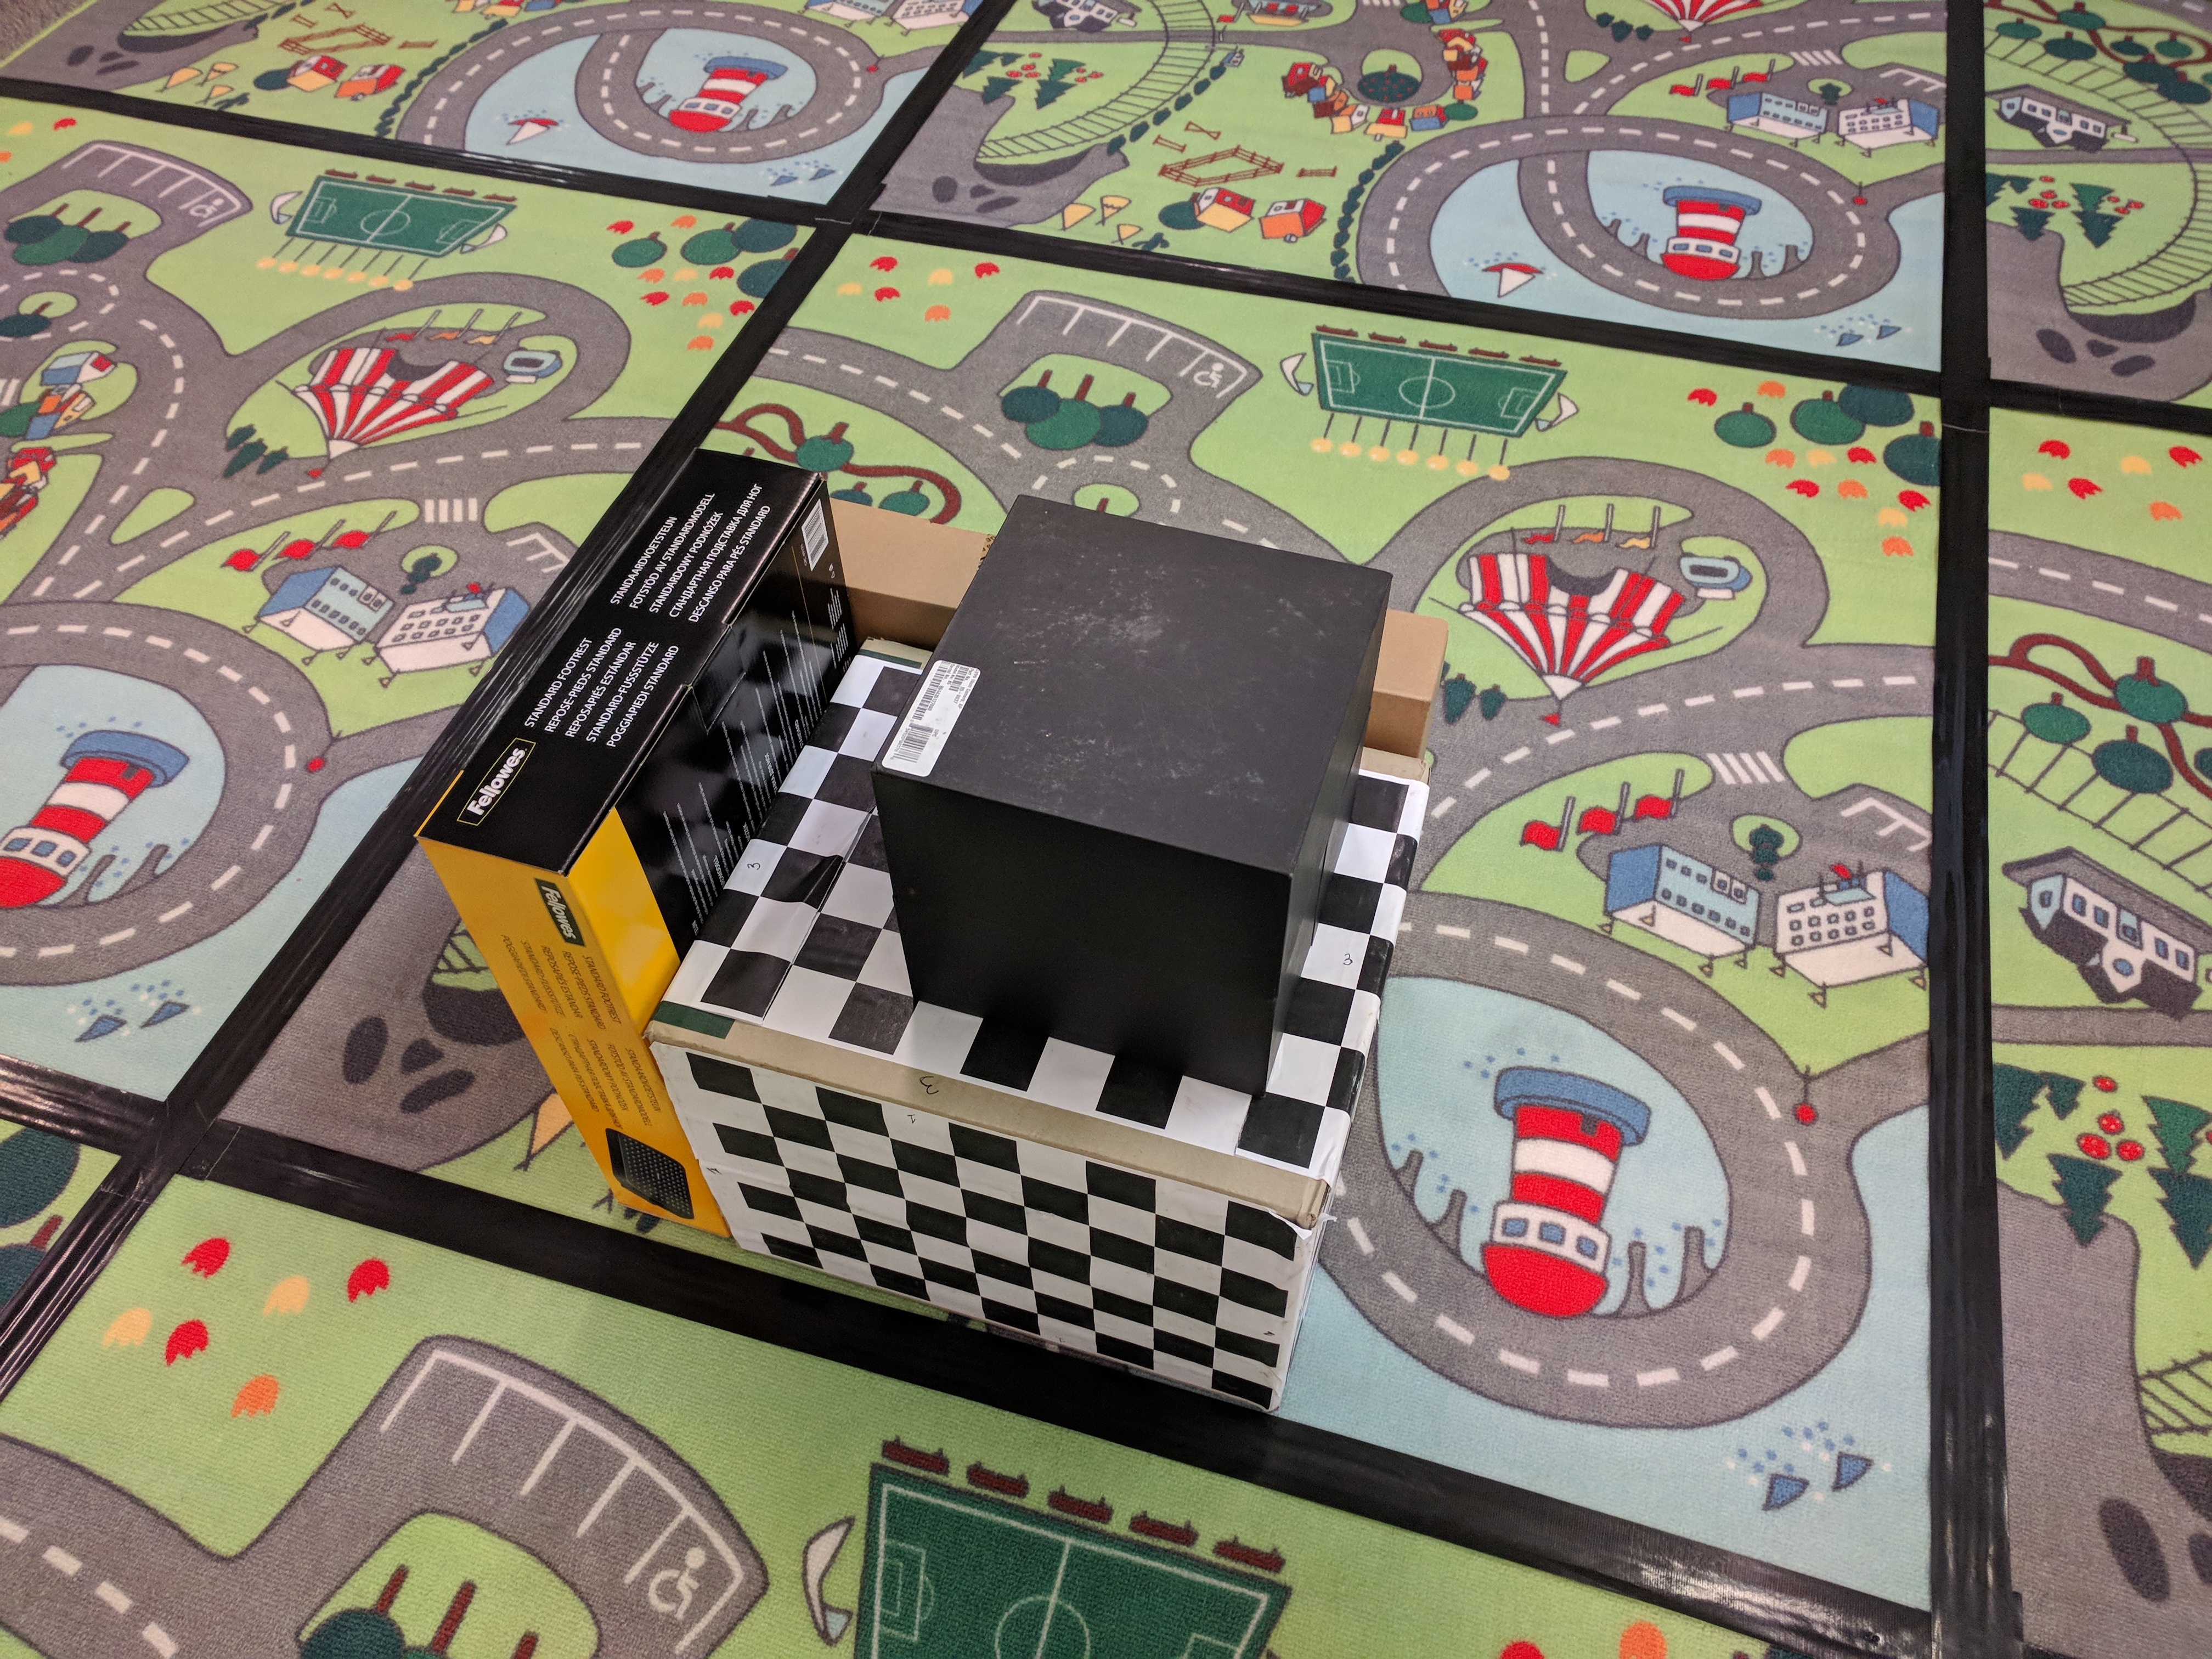
\includegraphics[width=50mm, trim =110mm 70mm 110mm 110mm, clip]{setup/IMG_20180518_140507.jpg}
      \caption{Set-up of scene for initial flight experiments}
      \label{f: initial setup}
    \end{figure}

    \begin{figure}[p]
      \begin{subfigure}[t]{0.5\textwidth}
      \centering
        \includegraphics[width=60mm]{box_test/cpp-headless-output-118_4_16_1_57_40_1526435860119.png}
      \caption{Box 1, RGB image}
      \end{subfigure}%
      ~
      \begin{subfigure}[t]{0.5\textwidth}
      \centering
        \includegraphics[width=60mm, trim =230mm 100mm 200mm 70mm, clip]{box_test/no_vicon1_36.png}
      \caption{Box 1, Point cloud}
      \end{subfigure}
      \\
      \begin{subfigure}[t]{0.5\textwidth}
      \centering
        \includegraphics[width=60mm]{box_test/cpp-headless-output-118_4_16_1_59_18_1526435958825.png}
      \caption{Box 2, RGB image}
      \end{subfigure} % 
       ~
      \begin{subfigure}[t]{0.5\textwidth}
      \centering
        \includegraphics[width=60mm, trim =50mm 50mm 50mm 20mm, clip]{box_test/no_vicon1_161.png}
      \caption{Box 2, Point cloud}
      \end{subfigure}
      \\
      \begin{subfigure}[t]{0.5\textwidth}
      \centering
        \includegraphics[width=60mm]{box_test/cpp-headless-output-118_4_16_2_0_59_1526436059005.png}
      \caption{Box 3, RGB image}
      \end{subfigure}%
      ~
      \begin{subfigure}[t]{0.5\textwidth}
      \centering
        \includegraphics[width=60mm, trim =50mm 50mm 50mm 50mm, clip]{box_test/no_vicon1_281.png}
      \caption{Box 3, Point cloud}
      \end{subfigure}
      \caption{RGB Image and Point cloud images for boxes, handheld RealSense R200 camera.}
      \label{f: box pcs}
    \end{figure}

    \begin{figure}[h]
      \centering
      \begin{subfigure}[t]{0.3\textwidth}
      \centering
        \includegraphics[width=45mm]{camera_tests/quad_camera_TX1}
      \caption{Depth image from R200 RealSense that was mounted to quadcopter, with code running on TX1}
      \end{subfigure} %
      ~
      \begin{subfigure}[t]{0.3\textwidth}
      \centering
        \includegraphics[width=45mm]{camera_tests/other_camera_TX1}
      \caption{Depth image from other R200 RealSense, with code running on TX1}
      \end{subfigure}%
      ~
      \begin{subfigure}[t]{0.3\textwidth}
      \centering
        \includegraphics[width=45mm]{camera_tests/other_camera_ubuntu}
      \caption{Depth image from other R200 RealSense, with code running on Ubuntu}
      \end{subfigure}
      \caption{Comparison of depth images for the two RealSense R200 cameras and for running on different platforms.}
      \label{f: R200 bad depth}
    \end{figure}


  % \subsection{Additional tables}

  % \subsection{Additional figures}

  \newpage
  \setminted{fontsize=\small,baselinestretch=1,tabsize=2}
  \subsection{Code: registration}
    \label{s: code reg}
    \begin{figure}[h]
      \centering
        \includegraphics[width=120mm]{diags/code_overview.PNG}
      \caption{Overview of registration code modules. Arrows show dependencies.}
      \label{f: code reg}
    \end{figure}  

  Figure \ref{f: code reg} shows the overview of the registration modules and how they relate to each other. run\_all is the main script that calls register and then uses functions from eval to display the trajectories (eval calls plotting to do the trajectory plots) and evaluate them. Both eval and register call functions in align\_timestamps to align the RGB, depth and ground truth data. align\_timestamps also has functions to convert from Euler angles to rotation matrices, as the ground truth orientation is given in Euler angles. register also calls im\_to\_cam in coord\_transforms to transform the 2D feature points and their associated depths into 3D points in the camera frame. kabsch implements the Kabsch data registration algorithm, with RANSAC, and is used by register. Note that the OpenCV implementations of the Essential Matrix method and PnP are used (by register). The code for each module is provided below.
   
  
  \noindent
  run\_all: 
  \inputminted{python}{../quad/run_all.py}

  \noindent
  register: 
  \inputminted{python}{../quad/register.py}

  \noindent
  coord\_transforms: 
  \inputminted{python}{../quad/coord_transforms.py}

  \noindent
  kabsch: 
  \inputminted{python}{../quad/kabsch.py}

  \noindent
  eval: 
  \inputminted{python}{../quad/eval.py}


  \noindent
  plotting: 
  \inputminted{python}{../quad/plotting.py}

  \noindent
  align\_timestamps: 
  \inputminted{python}{../quad/align_timestamps.py}


  \subsection{Code: flying}
    \label{a: code flying}
    The code for the trajectories is written in C as part of a ROS package. A separate file is written for each trajectory, which will be provided below.

    \noindent
    Circle:
    \inputminted{cpp}{../trj_code/circle/vicon_test.cpp}
    
    \noindent
    Rectangle:
    \inputminted{cpp}{../trj_code/rectangle/vicon_test.cpp}

    \noindent
    Lawnmower:
    \inputminted{cpp}{../trj_code/lawnmower/vicon_test.cpp}

\end{document}